\pdfoptionpdfminorversion=5
\documentclass[hyperref={pdfpagelabels=false},10pt,gray]{beamer}
\usepackage[utf8]{inputenc}
\usepackage[english,russian]{babel}
\usepackage{amssymb,amsfonts,amsmath,mathtext}
\usepackage{cite,enumerate,float,indentfirst}
\usepackage{listings}
 
\usepackage{tikz}
\usetikzlibrary{positioning,arrows,matrix}

\lstdefinestyle{customc}{
  belowcaptionskip=1\baselineskip,
  breaklines=true,
  frame=L,
  xleftmargin=\parindent,
  language=C,
  showstringspaces=false,
  basicstyle=\ttfamily,
  keywordstyle=\bfseries\color{green!40!black},
  commentstyle=\itshape\color{purple!40!black},
  identifierstyle=\color{blue},
  stringstyle=\color{orange},
  numbers=left,
}

\lstset{escapechar=@,style=customc}


\graphicspath{{images/}}

%\usetheme{Pittsburgh}
%\usecolortheme{whale}

% \usepackage[defaultsans]{opensans}
% \renewcommand*\familydefault{\sfdefault} %% Only if the base font of the document is to be typewriter style
\usepackage[T2A]{fontenc}

\newcommand{\itemi}{\item[\checkmark]}
\setbeamercolor{frametitle}{fg=black}
\title{Метод межпроцедурного и межмодульного анализа кодов программ, написанных на~языках  С и С++}

\begin{document}


\begin{frame}
  \center{\Huge{Метод межпроцедурного\\и~межмодульного анализа кодов программ, написанных на~языках  С и С++}}
\end{frame}

%--------------------------------------------------------------------------------------------------------
\begin{frame}
\frametitle{Cложные программные системы}
\begin{figure}[h]
  \center{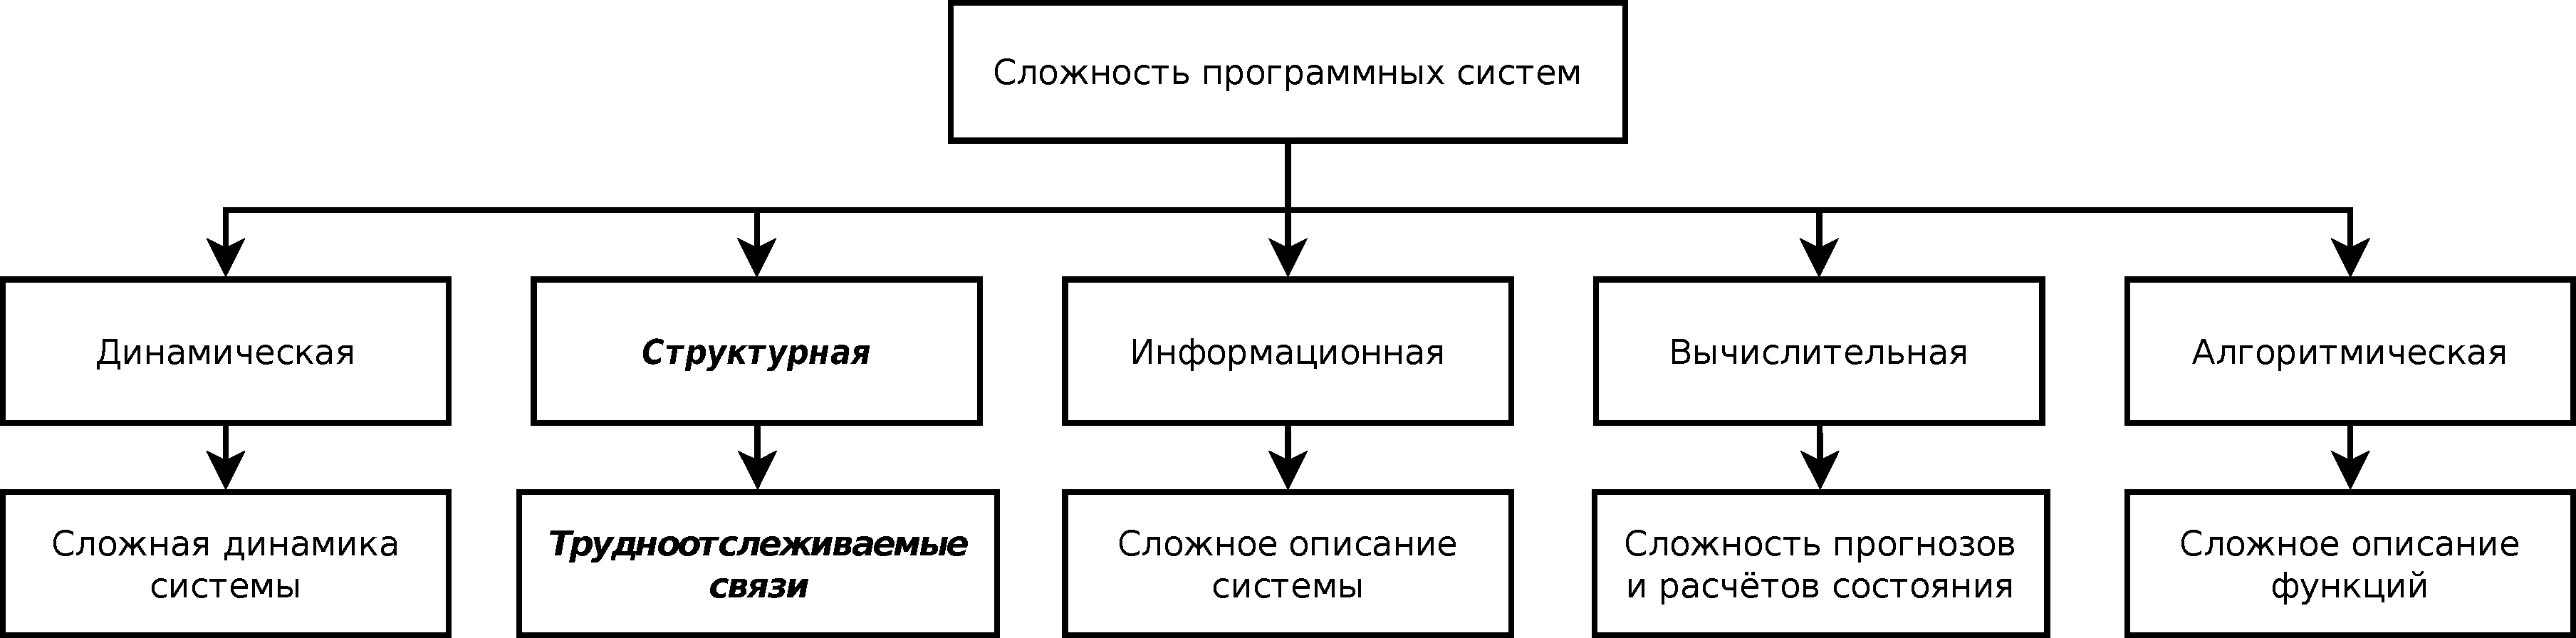
\includegraphics[width=\linewidth]{../Dissertation/images/complexity-1.pdf}}
\end{figure}
\end{frame}
%--------------------------------------------------------------------------------------------------------
\renewcommand{\arraystretch}{1.2}


\begin{frame}
\frametitle{Актуальность проблемы анализа программных систем}
\begin{figure}[h]
    \center{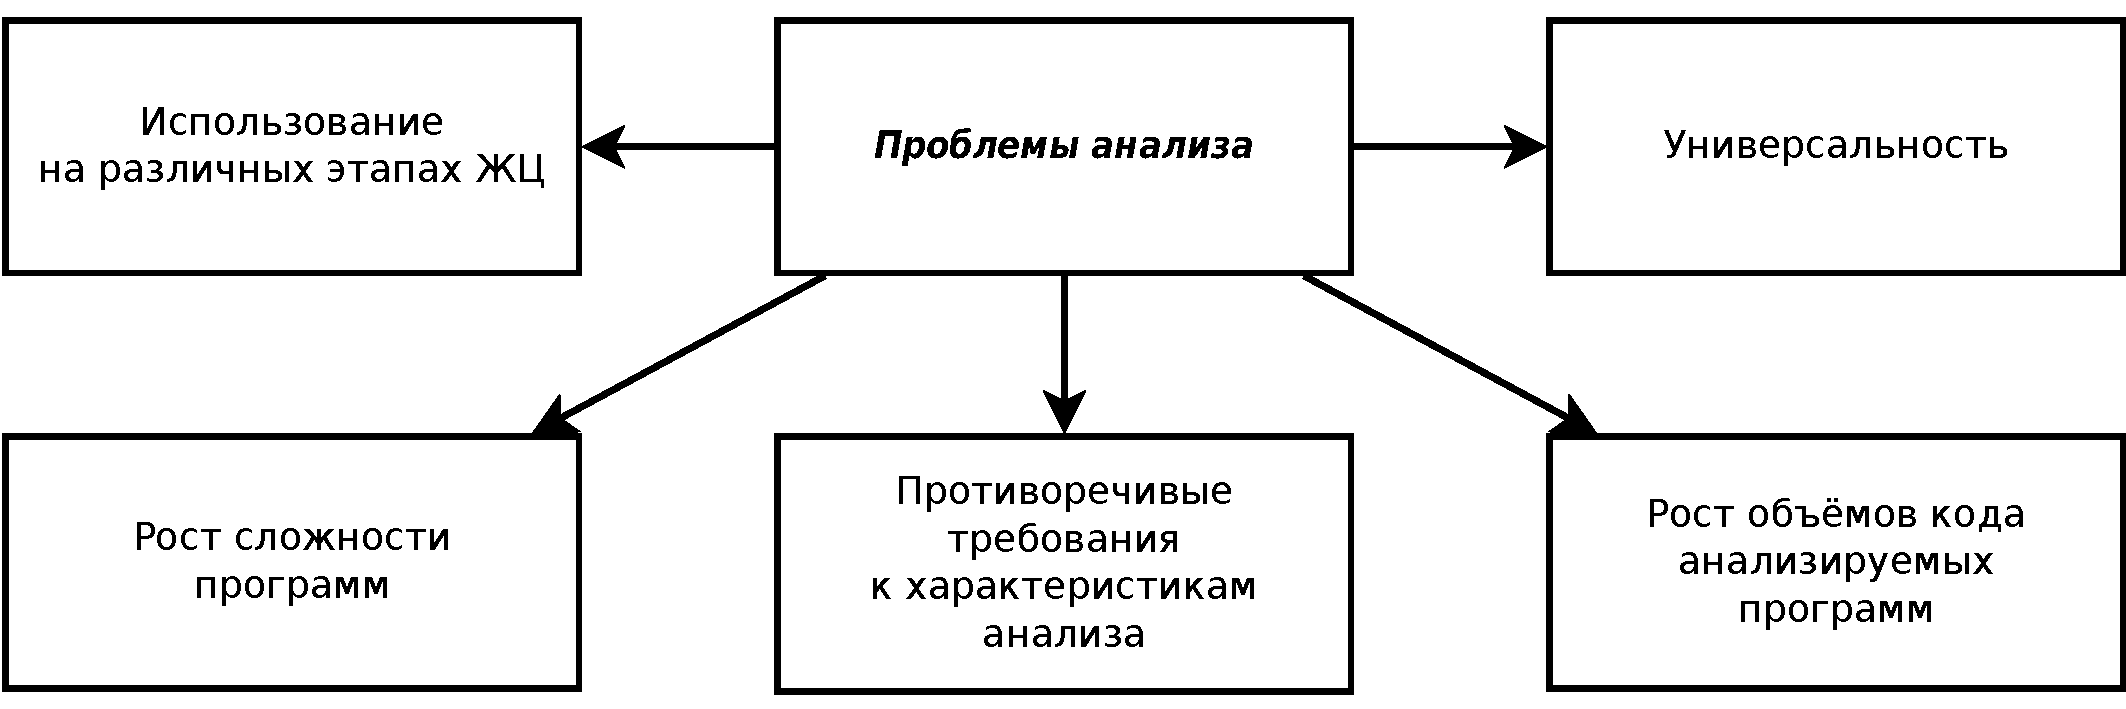
\includegraphics[width=1\linewidth]{../Dissertation/images/problems.pdf}}
    
    \textbf{ЖЦ безопасного ПО}
    \center{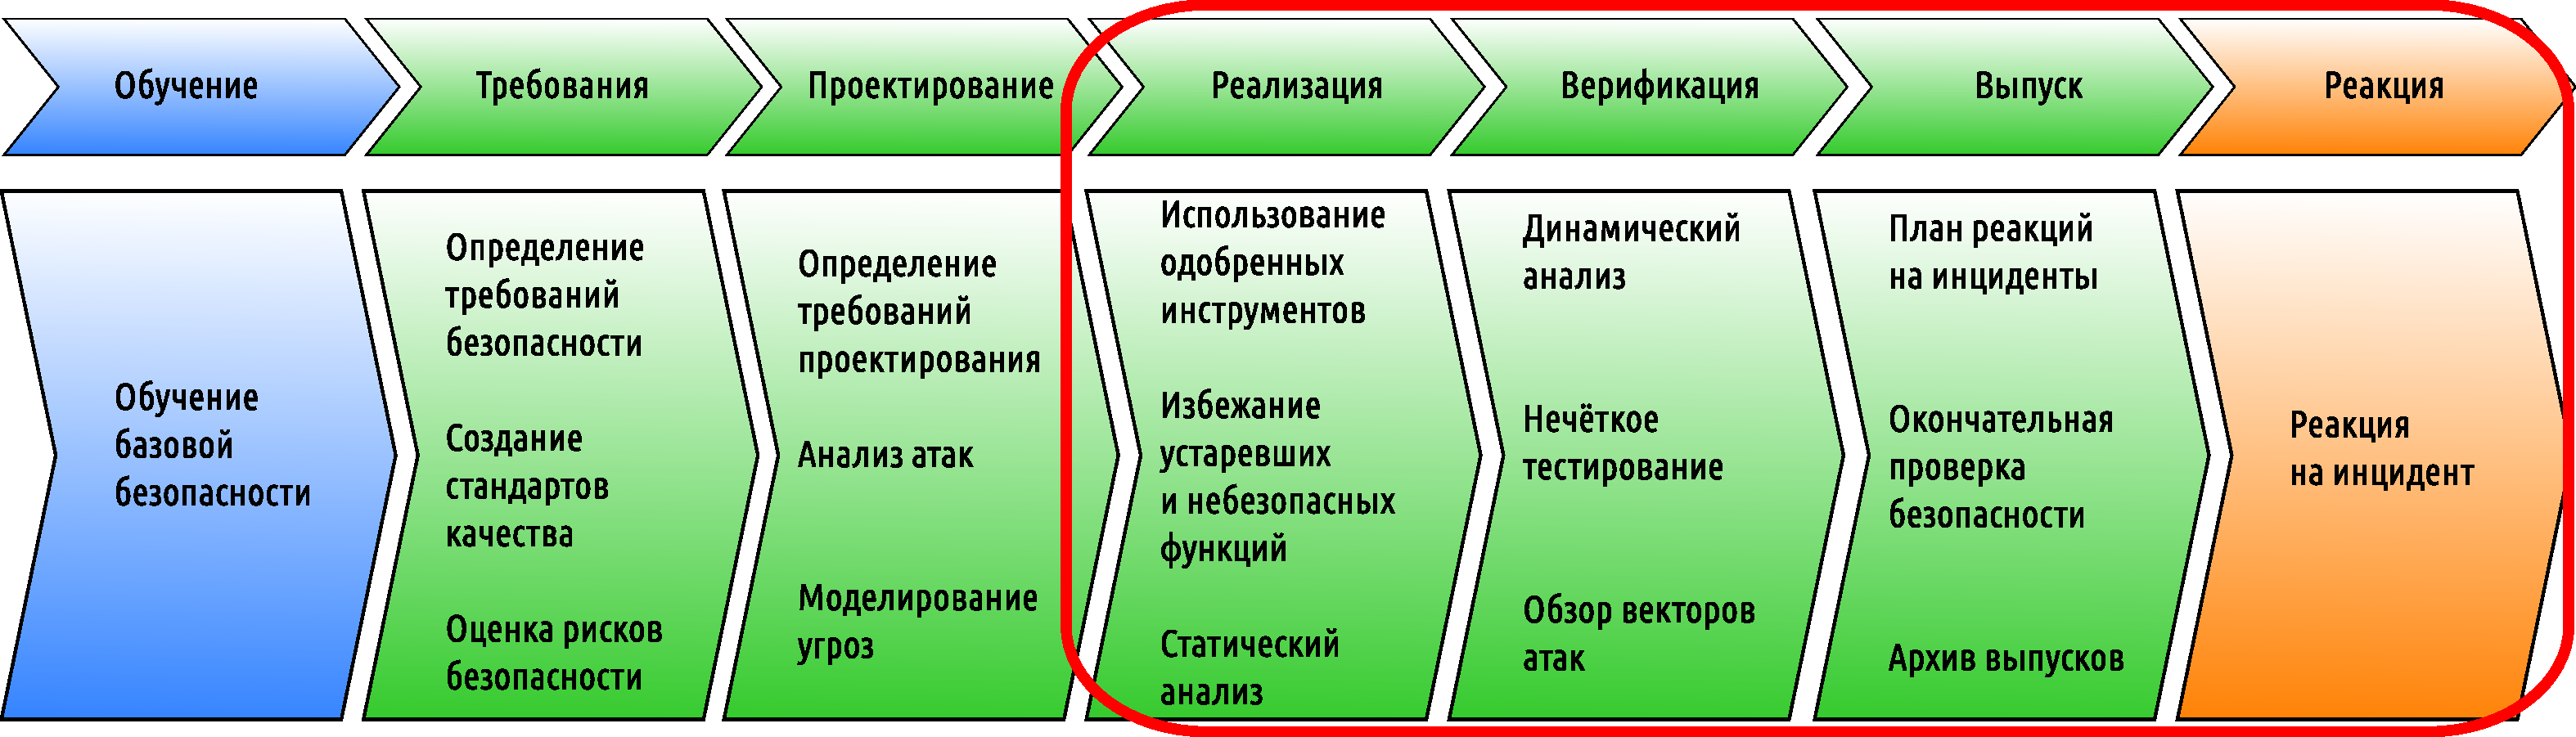
\includegraphics[width=1\linewidth]{../Dissertation/images/ms-sdl-sel.pdf}}

\end{figure}
\end{frame}

%--------------------------------------------------------------------------------------------------------
% \begin{frame}[fragile]
% %TODO: Разделить практические и теоретические работы
% %TODO: Дополнить список, в т.ч. отечественными работами (CEGAR)
% \frametitle{Наиболее известные работы, относящиеся к методу символьного выполнения:}
% \begin{enumerate}
%  \item J. King, 1976. Symbolic Execution and Program Testing.
%  \item P. Godefroid, 2007. Compositional Dynamic Test Generation.
%  \item V.~Kuznetsov, J.~Kinder, S.~Bucur, G.~Candea, 2012. Efficient State Merging in Symbolic Execution.
%  \item  Anand Saswat, 2012. Techniques to Facilitate Symbolic Execution of Real-World Programs.
%  \item Sang Kil Cha, T. Avgerinos, A. Rebert, D. Brumley, 2012 Unleashing Mayhem on Binary Code.
%  \item A. Ibing, 2014. Demand-driven Compositional Symbolic Execution.
% \end{enumerate}
\end{frame}
%--------------------------------------------------------------------------------------------------------

\begin{frame}
%\frametitle{Цель работы}
\textbf{\Large{Цель работы}}. Разработать методы межпроцедурного и межмодульного анализа сложных программных систем, написанных на языках C и C++, для автоматического поиска дефектов различных видов, и реализация программного обеспечения для статического анализа кодов программ на основе этих методов.

%\end{frame}
\vspace{5pt}
%\begin{frame}[allowframebreaks]
\textbf{\Large{Решаемые задачи}}

\begin{enumerate}
  \item Разработка модификации метода межпроцедурного анализа программ, пригодной для реализации в многоцелевом статическом анализаторе программного кода на языках C и C++ и позволяющей использовать различные виды проверок кода с целью поиска дефектов.
  \item Разработка метода межмодульного анализа программ, реализованных с использованием языков C и C++, для повышения полноты анализа многокомпонентных систем.
  \item Реализация программного обеспечения (многоцелевой анализатор и его утилиты) на основе предложенных методов с целью его промышленного и коммерческого применения для поиска дефектов в исходном коде программных комплексов.
\end{enumerate}

\end{frame}

%--------------------------------------------------------------------------------------------------------

\begin{frame}
\frametitle{Межпроцедурный анализ}
\begin{figure}[h]
  \center{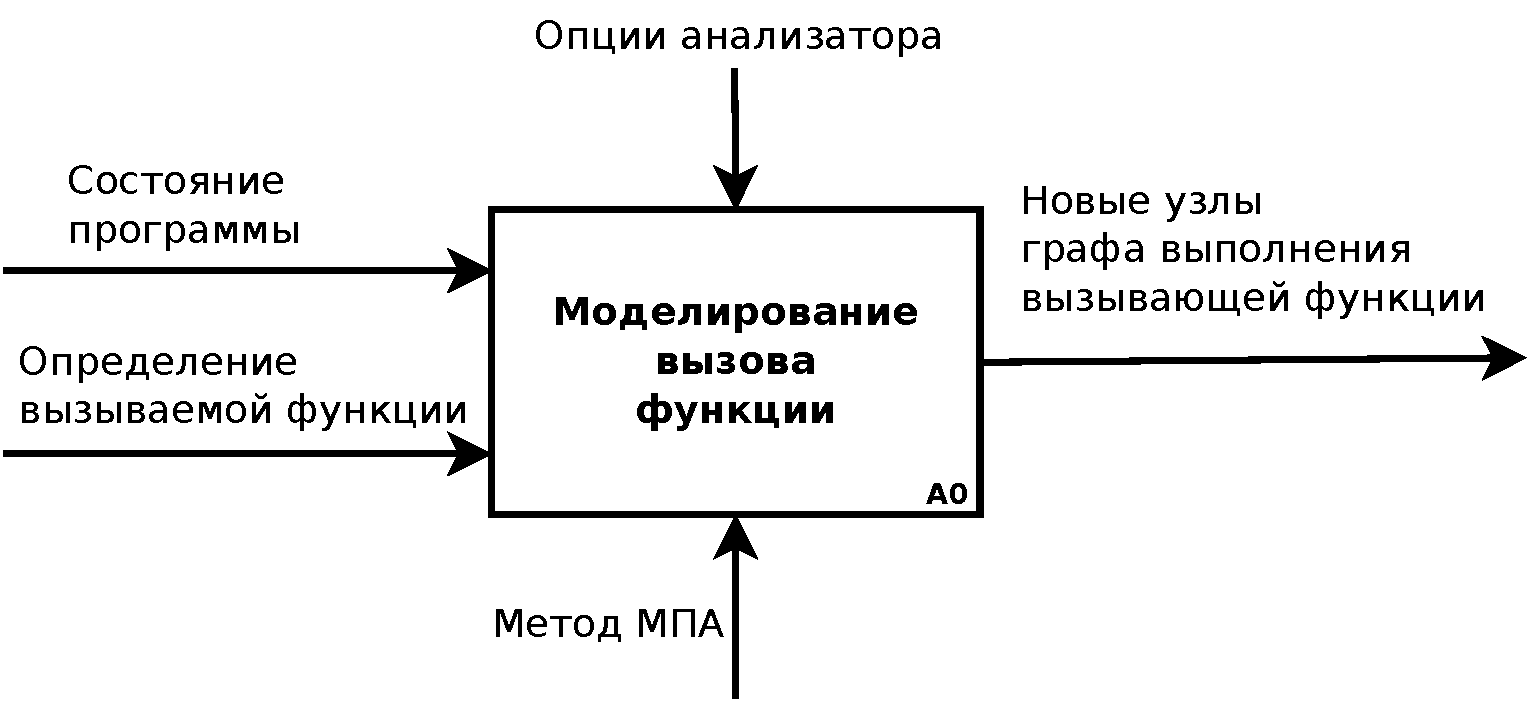
\includegraphics[width=1\linewidth]{../Dissertation/images/ipa-idef0-hl.pdf}}
\end{figure}
\end{frame}

%--------------------------------------------------------------------------------------------------------

\begin{frame}
\frametitle{Межпроцедурный анализ с помощью резюме}
\begin{figure}[h]
  \center{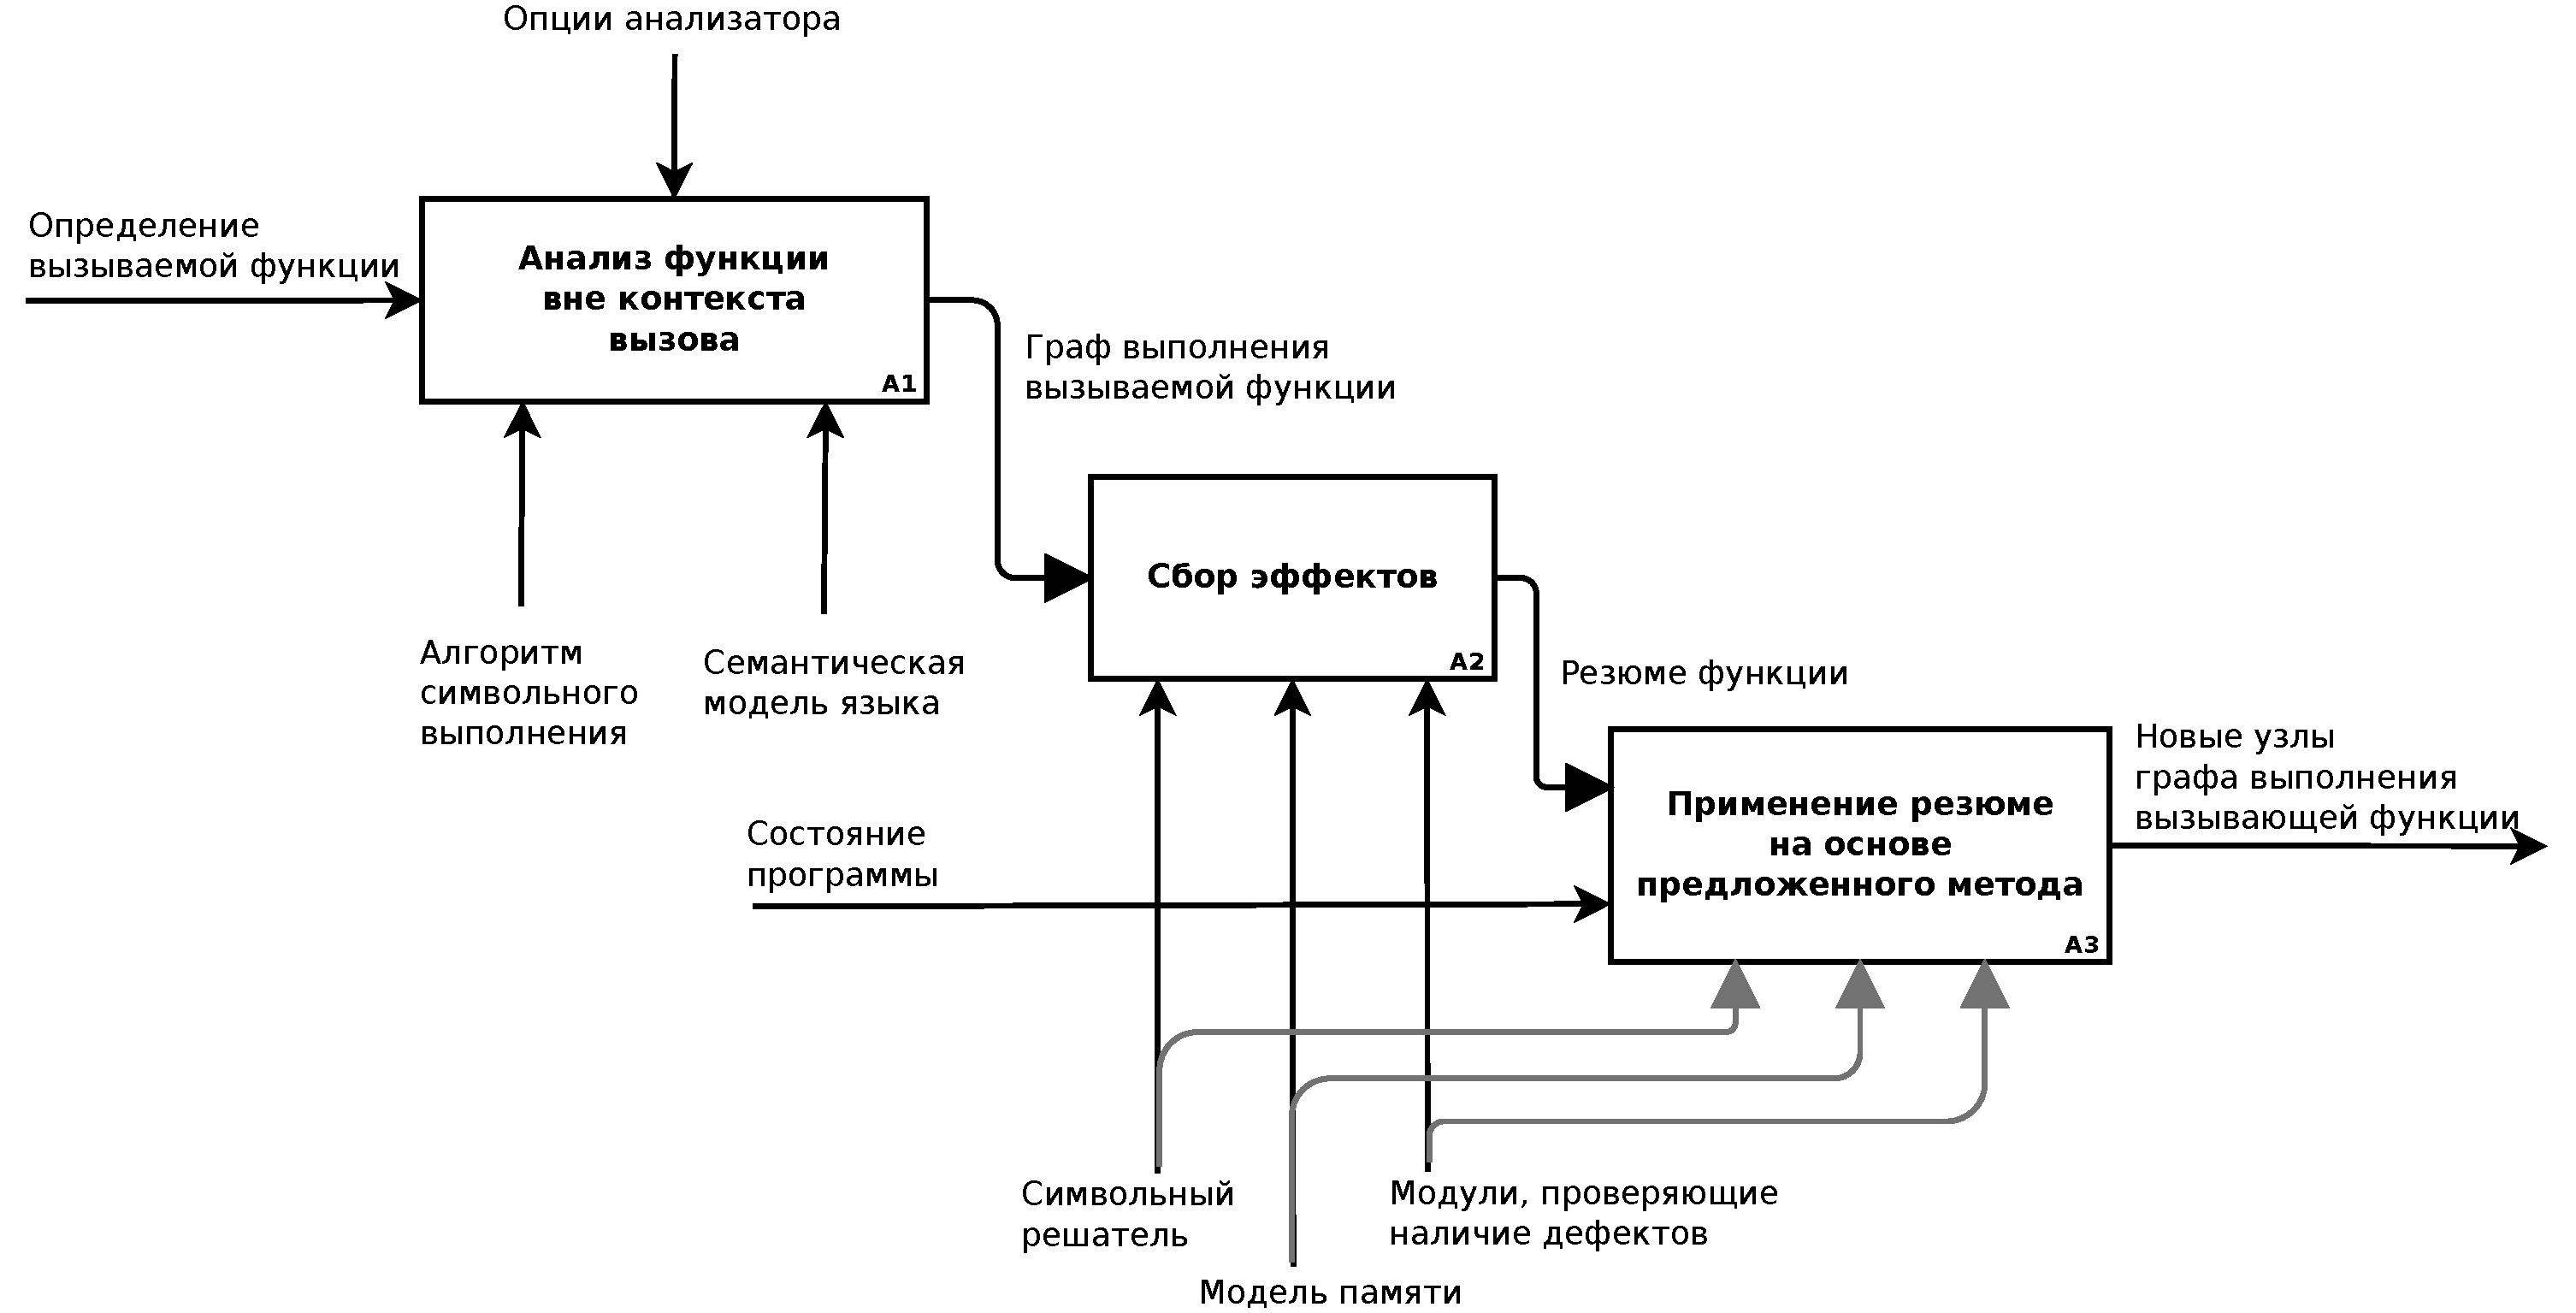
\includegraphics[width=1\linewidth]{../Dissertation/images/summary-idef0-ll.pdf}}
\end{figure}
\end{frame}
%--------------------------------------------------------------------------------------------------------

% \begin{frame}
% \frametitle{Межпроцедурный анализ с помощью резюме}
% \begin{figure}[h]
%   \center{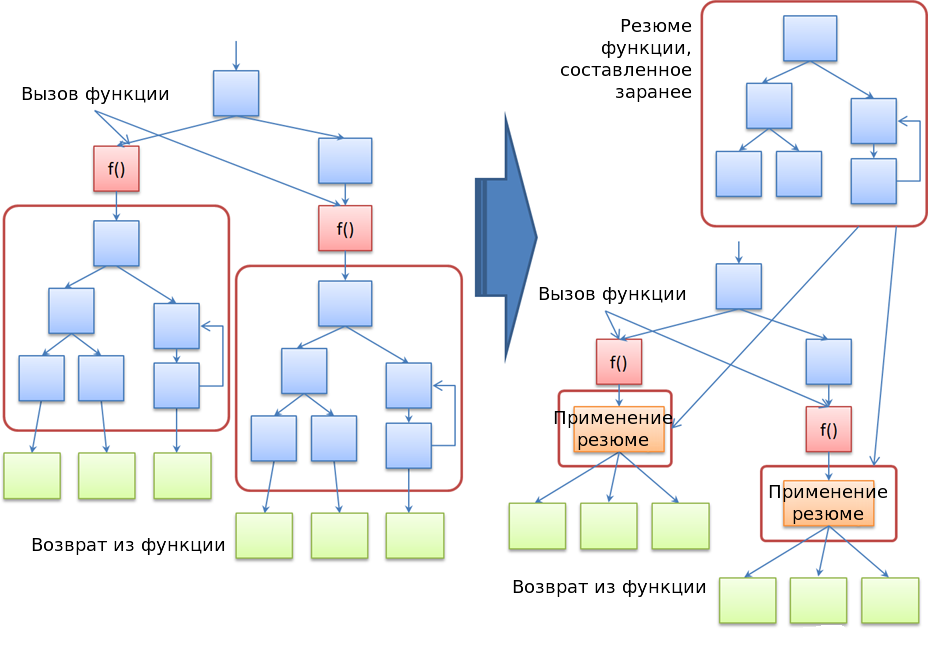
\includegraphics[width=1\linewidth]{images/summary.png}}
% \end{figure}
% \end{frame}

%--------------------------------------------------------------------------------------------------------

\begin{frame}
\frametitle{Учитываемые эффекты выполнения функции\\в методе межпроцедурного анализа на~основе резюме}
В резюме функции сохраняются следующие эффекты, влияющие на состояние программы:
\begin{figure}[h]
  \center{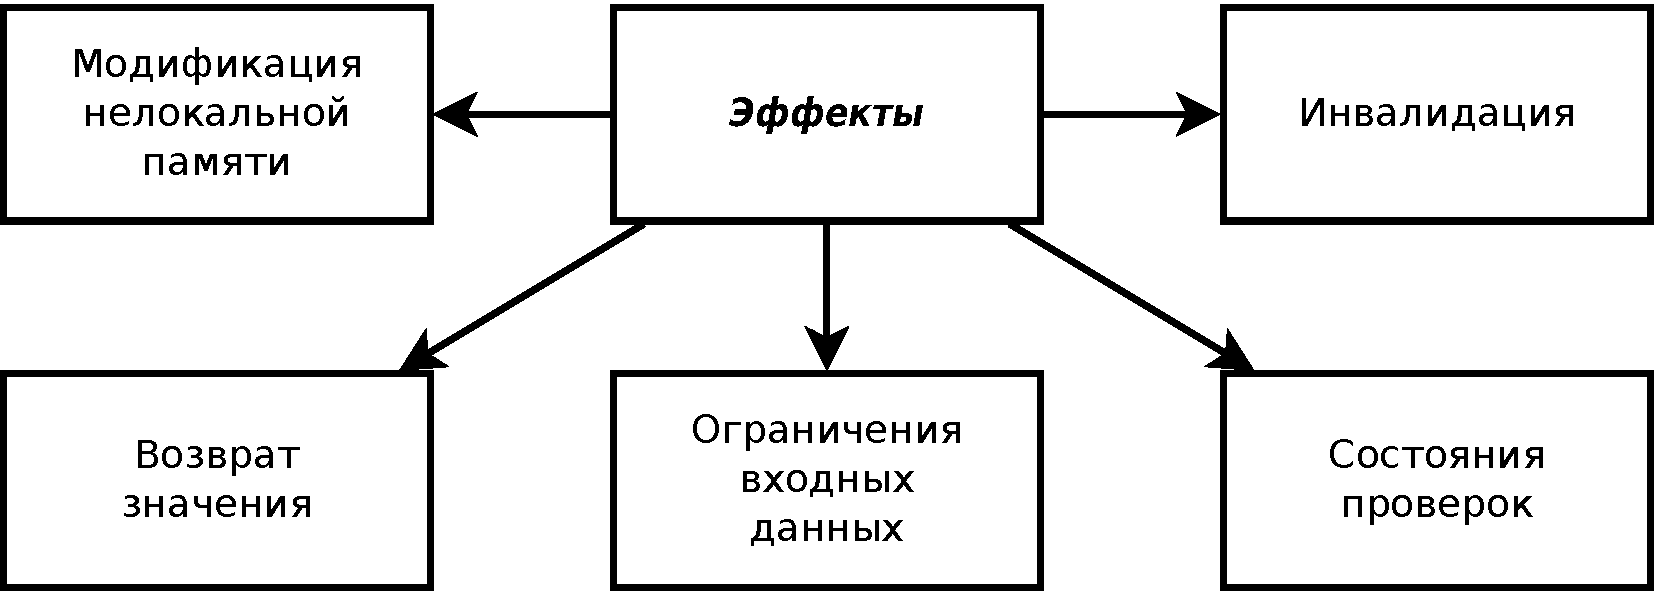
\includegraphics[width=1\linewidth]{../Dissertation/images/effects.pdf}}
\end{figure}
\end{frame}
%--------------------------------------------------------------------------------------------------------

\begin{frame}
\frametitle{Последовательность применения резюме}
\begin{figure}[h]
  \center{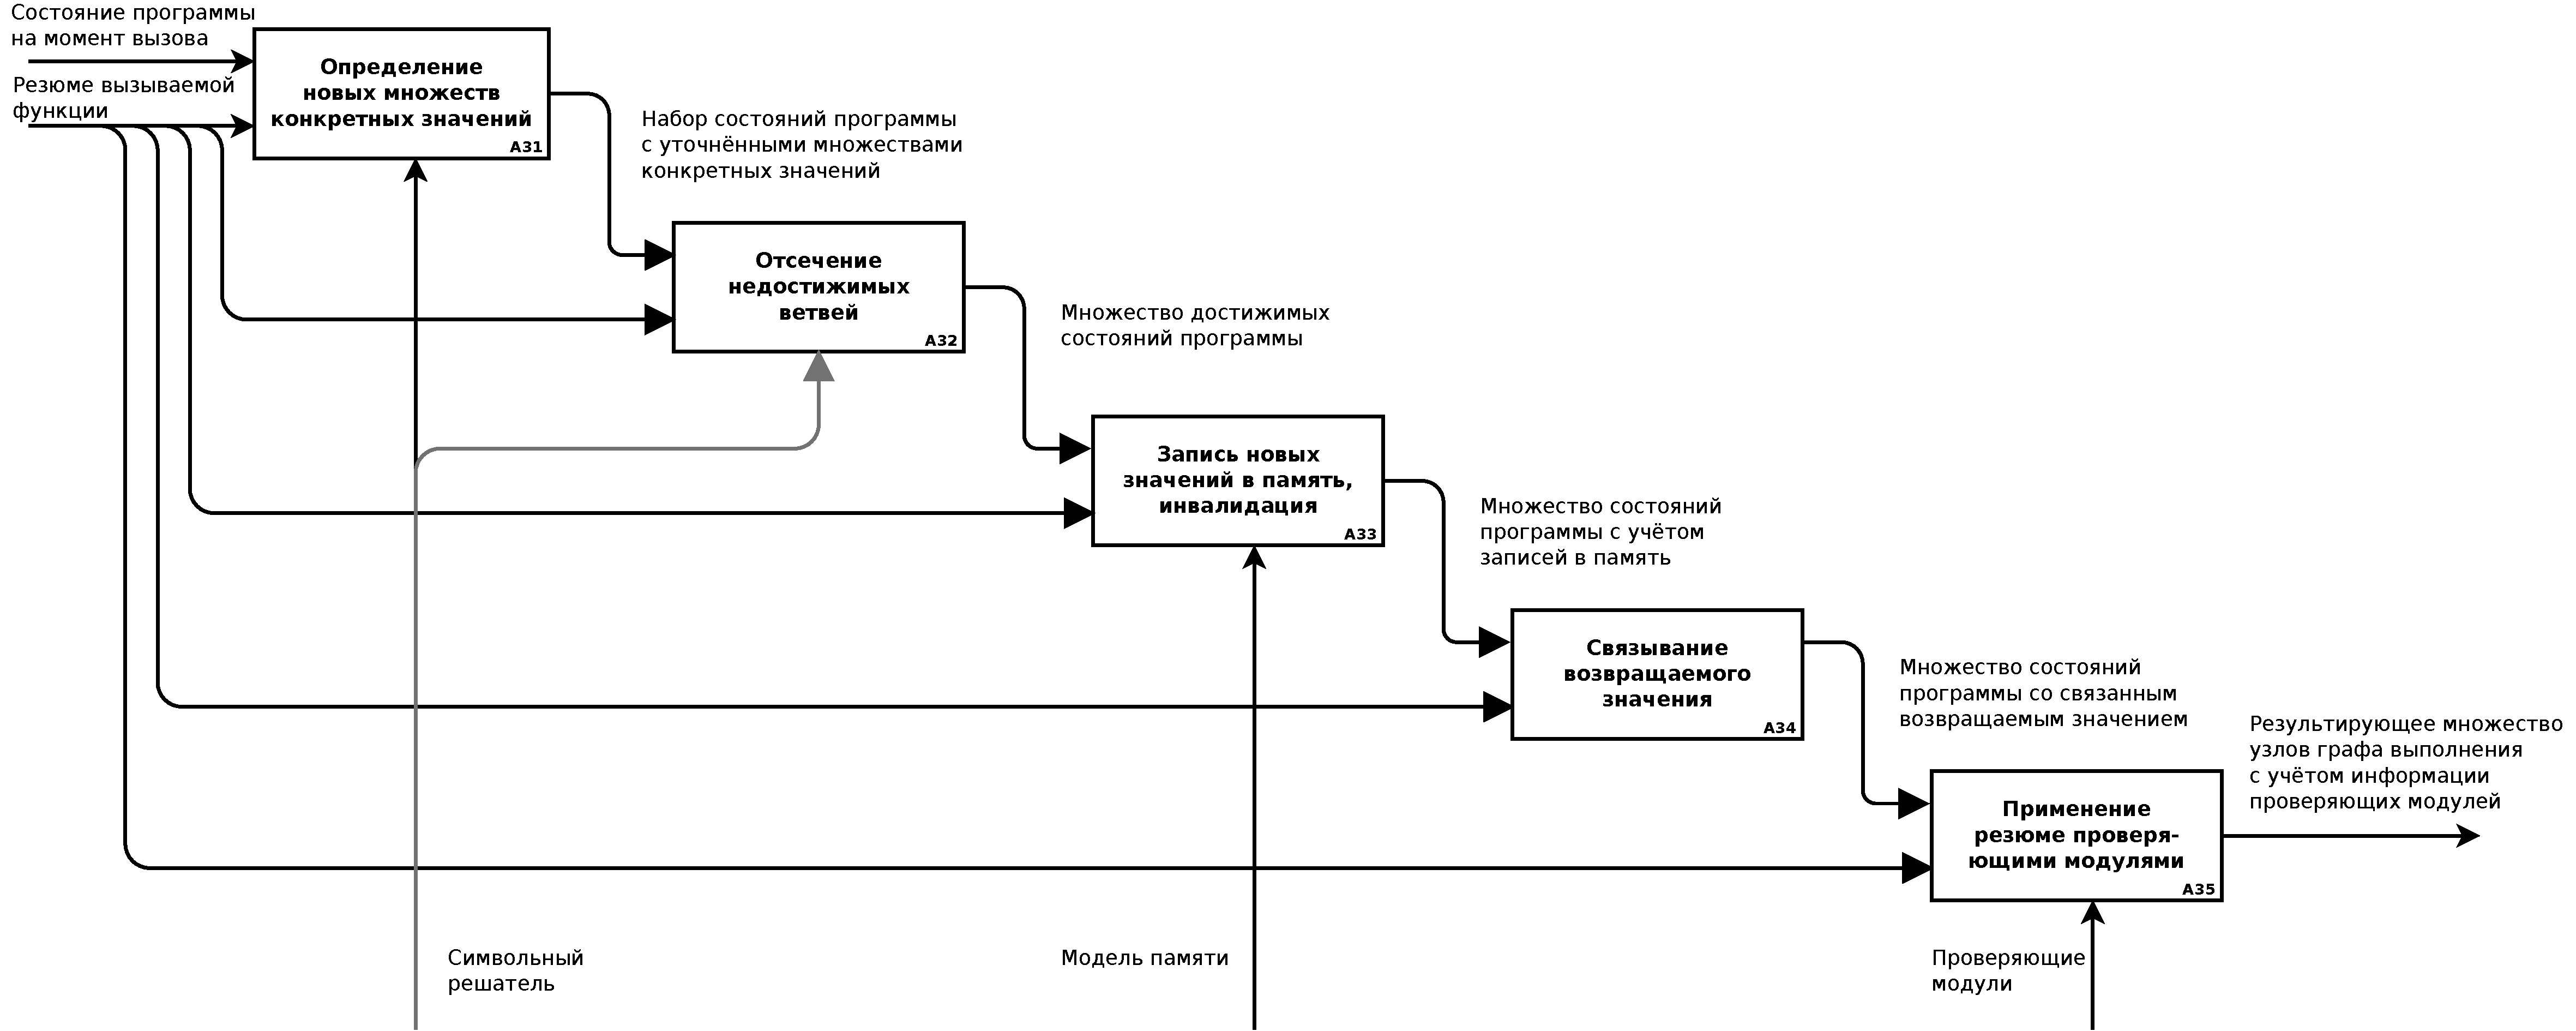
\includegraphics[width=1\linewidth]{../Dissertation/images/summary-apply.pdf}}
\end{figure}
\end{frame}
%--------------------------------------------------------------------------------------------------------

\begin{frame}
\frametitle{Достижимость ветвей в графе выполнения программы}

\textbf{Формализация предусловий, позволяющих выделить и уточнить условия в достижимых ветвях графа выполнения и убрать из рассмотрения недостижимые, описывается с помощью следующих формальных правил: }

\vspace{20pt}

Расчёт нового множества конкретных значений $R_{ij}$ для символьного значения $j$ в ветви выполнения $i$:
\begin{equation*}
\label{result_sval}
 \forall i \in [0; n], \forall j \in [0; p_i]:\ R_{\text{выходные}\ ij} =  R_{\text{входные}\ ij} \cap R_{\text{резюме}\ ij},
\end{equation*}
Отсечение недостижимых ветвей:
\begin{equation*}
 \label{empty_set}
 (\exists i, j: R_{\text{входные}\ ij} \cap R_{\text{резюме}\ ij} = \varnothing)  \Rightarrow (state_{\text{входное}} \nrightarrow state_{\text{выходное}}),
\end{equation*}
$n$~--- количество ветвей в графе выполнения,

$p_{i}$~--- количество символьных значений в $i$-й ветви выполнения.


\end{frame}

%--------------------------------------------------------------------------------------------------------

\begin{frame}
\frametitle{Поиск соответствия между регионами памяти}
Процесс актуализации регионов памяти заключается в построении цепочки доступа и поиске соответствия между базовыми регионами.
\vspace{10pt}

$Mem := Base\_Mem(F|E|P)^*$

\vspace{10pt}

$F$~--- член структуры или класса\\
$E$~--- элемент массива\\
$P$~--- регион, которому соответствует указатель или ссылка

\vspace{10pt}

$Base\_Mem := Var|This|Temp$

\vspace{10pt}

$Var$~--- переменная\\
$This$~--- регион текущего объекта (\texttt{*this})\\
$Temp$~--- регион временного объекта


\end{frame}

%--------------------------------------------------------------------------------------------------------

\begin{frame}
\frametitle{Актуализация символьных значений}

\begin{enumerate}
 \item Для всех регионов памяти, содержащихся в символьном значении:
 \begin{enumerate}
  \item Определить регион, соответствующий данному региону в вызывающей функции
  \item Заменить в символьном значении исходный регион актуализированным
 \end{enumerate}
 \item Для всех символов, содержащихся в символьном значении, полученном на шаге 1:
  \begin{enumerate}
  \item Проверить, не вычисляется ли символ в константу
  \item Если символ вычисляется в константу, заменить данный символ вычисленной константой.
 \end{enumerate}

\end{enumerate}
\end{frame}

%--------------------------------------------------------------------------------------------------------

\begin{frame}
\frametitle{Построение отчёта произвольной вложенности}
Отчёт строится с помощью последовательного движения по графам выполнения вызываемой и вызывающей функции.

При хранении всего стека применения резюме можно строить отчёты произвольной вложенности.
\begin{figure}[h]
  \center{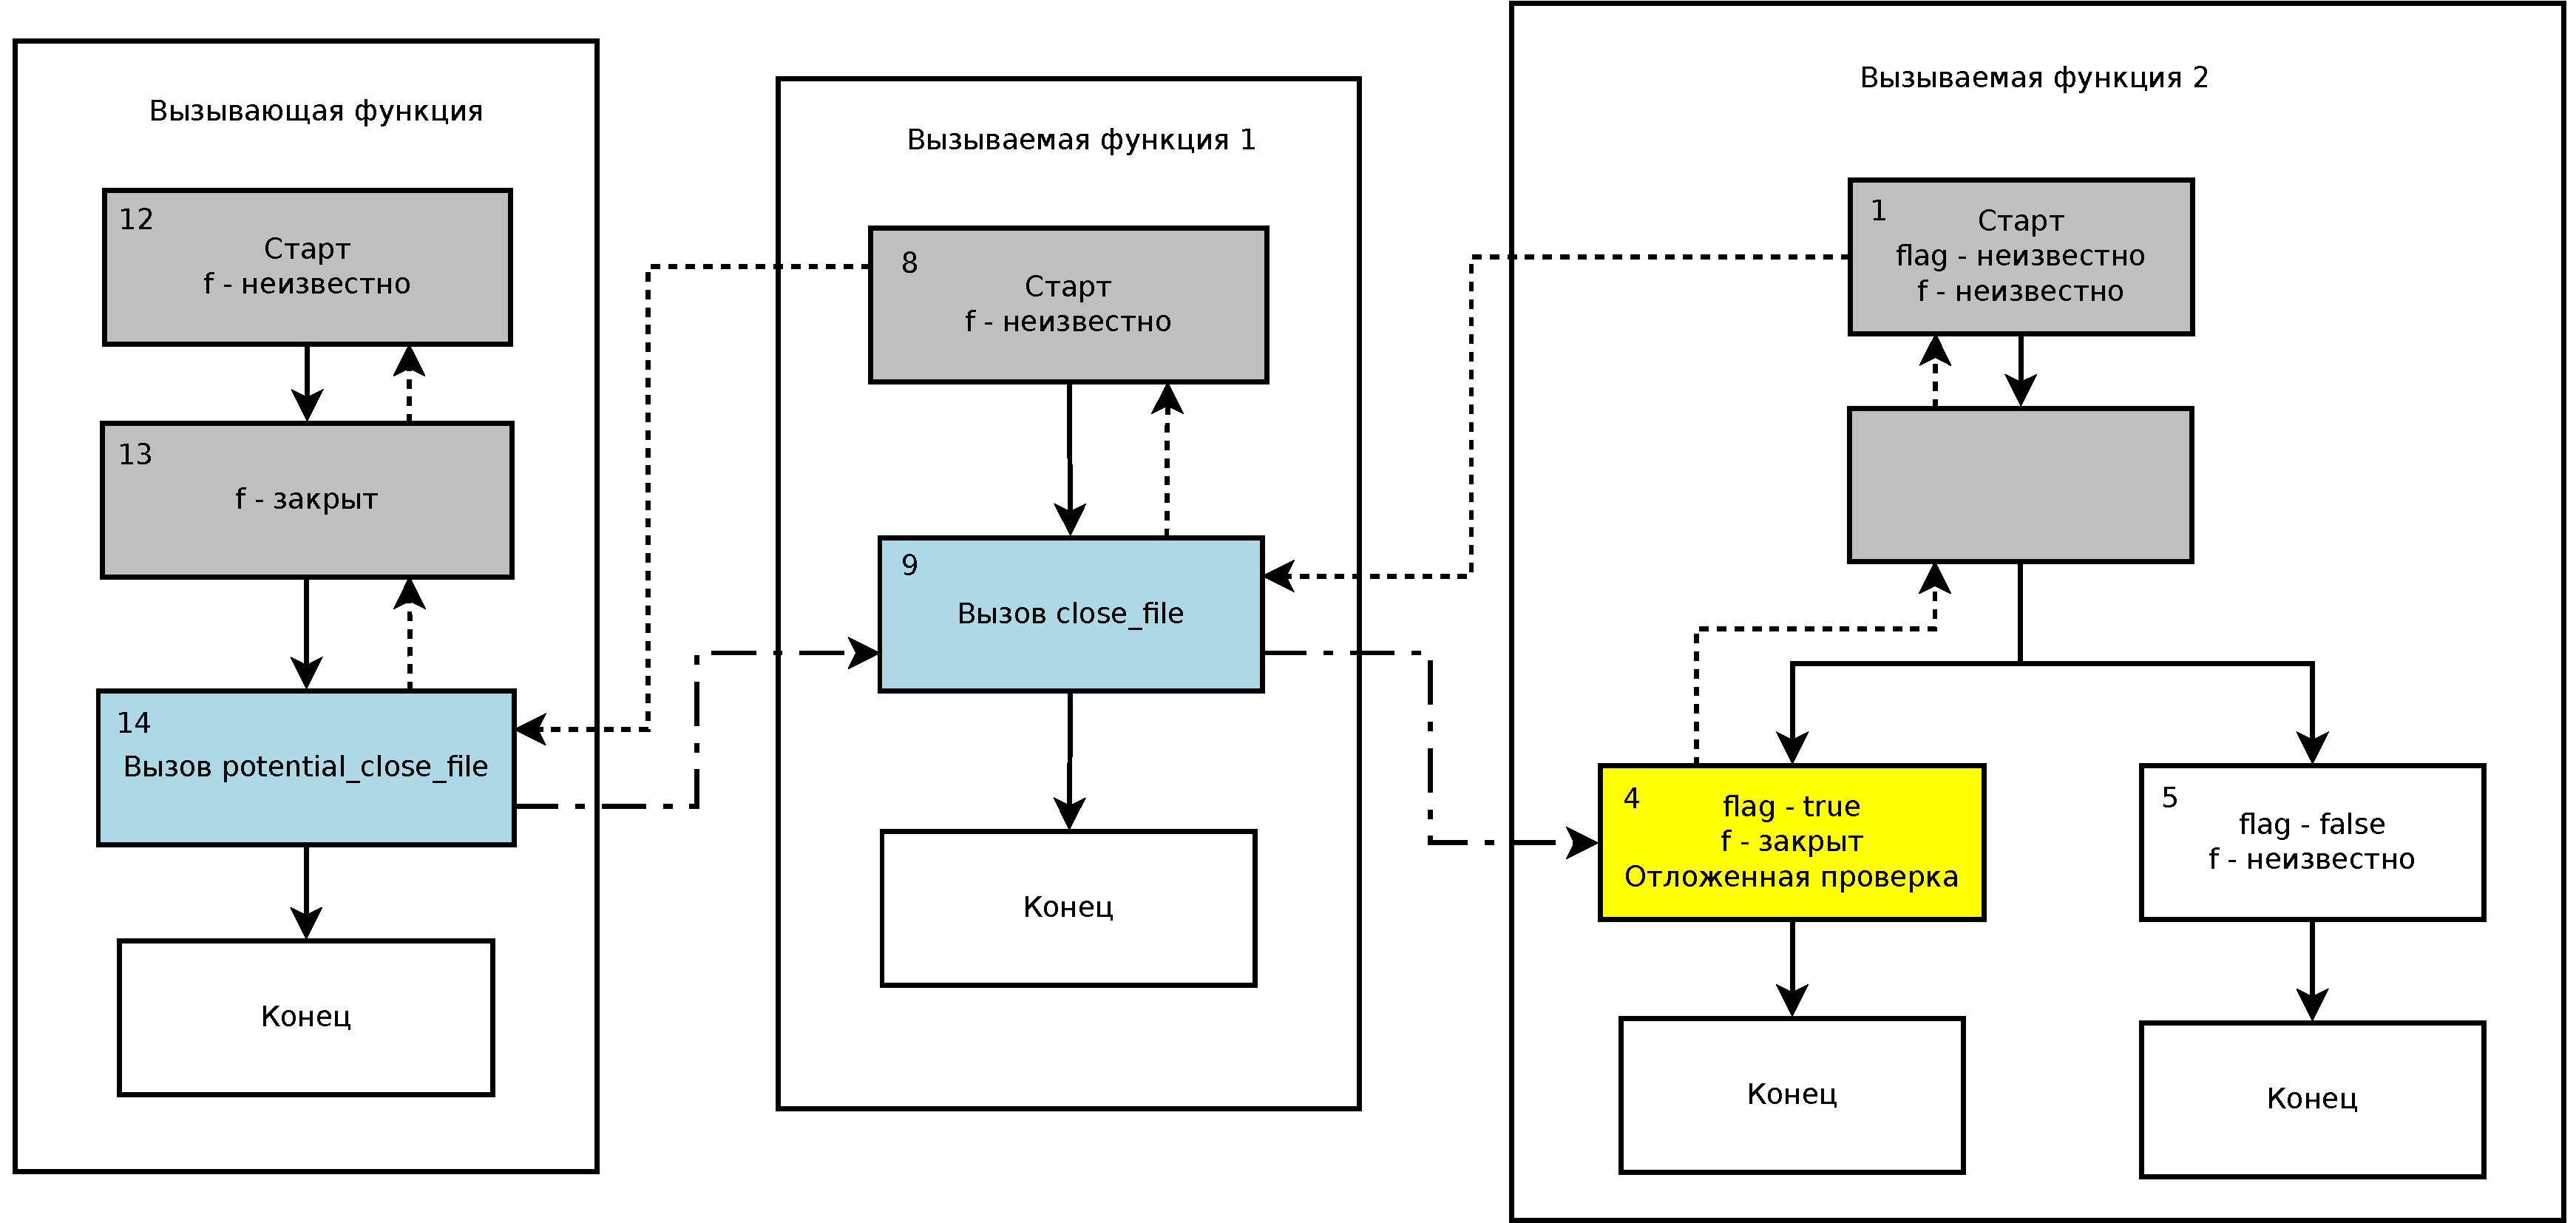
\includegraphics[width=1\linewidth]{../Dissertation/images/call-trace-multiple-2.pdf}}
\end{figure}
\end{frame}


%--------------------------------------------------------------------------------------------------------

\begin{frame}
\frametitle{Межмодульный анализ}
Функциональная модель межмодульного анализа, используемая в разработанном ПО, представлена в нотации IDEF0.
\begin{figure}[h]
  \center{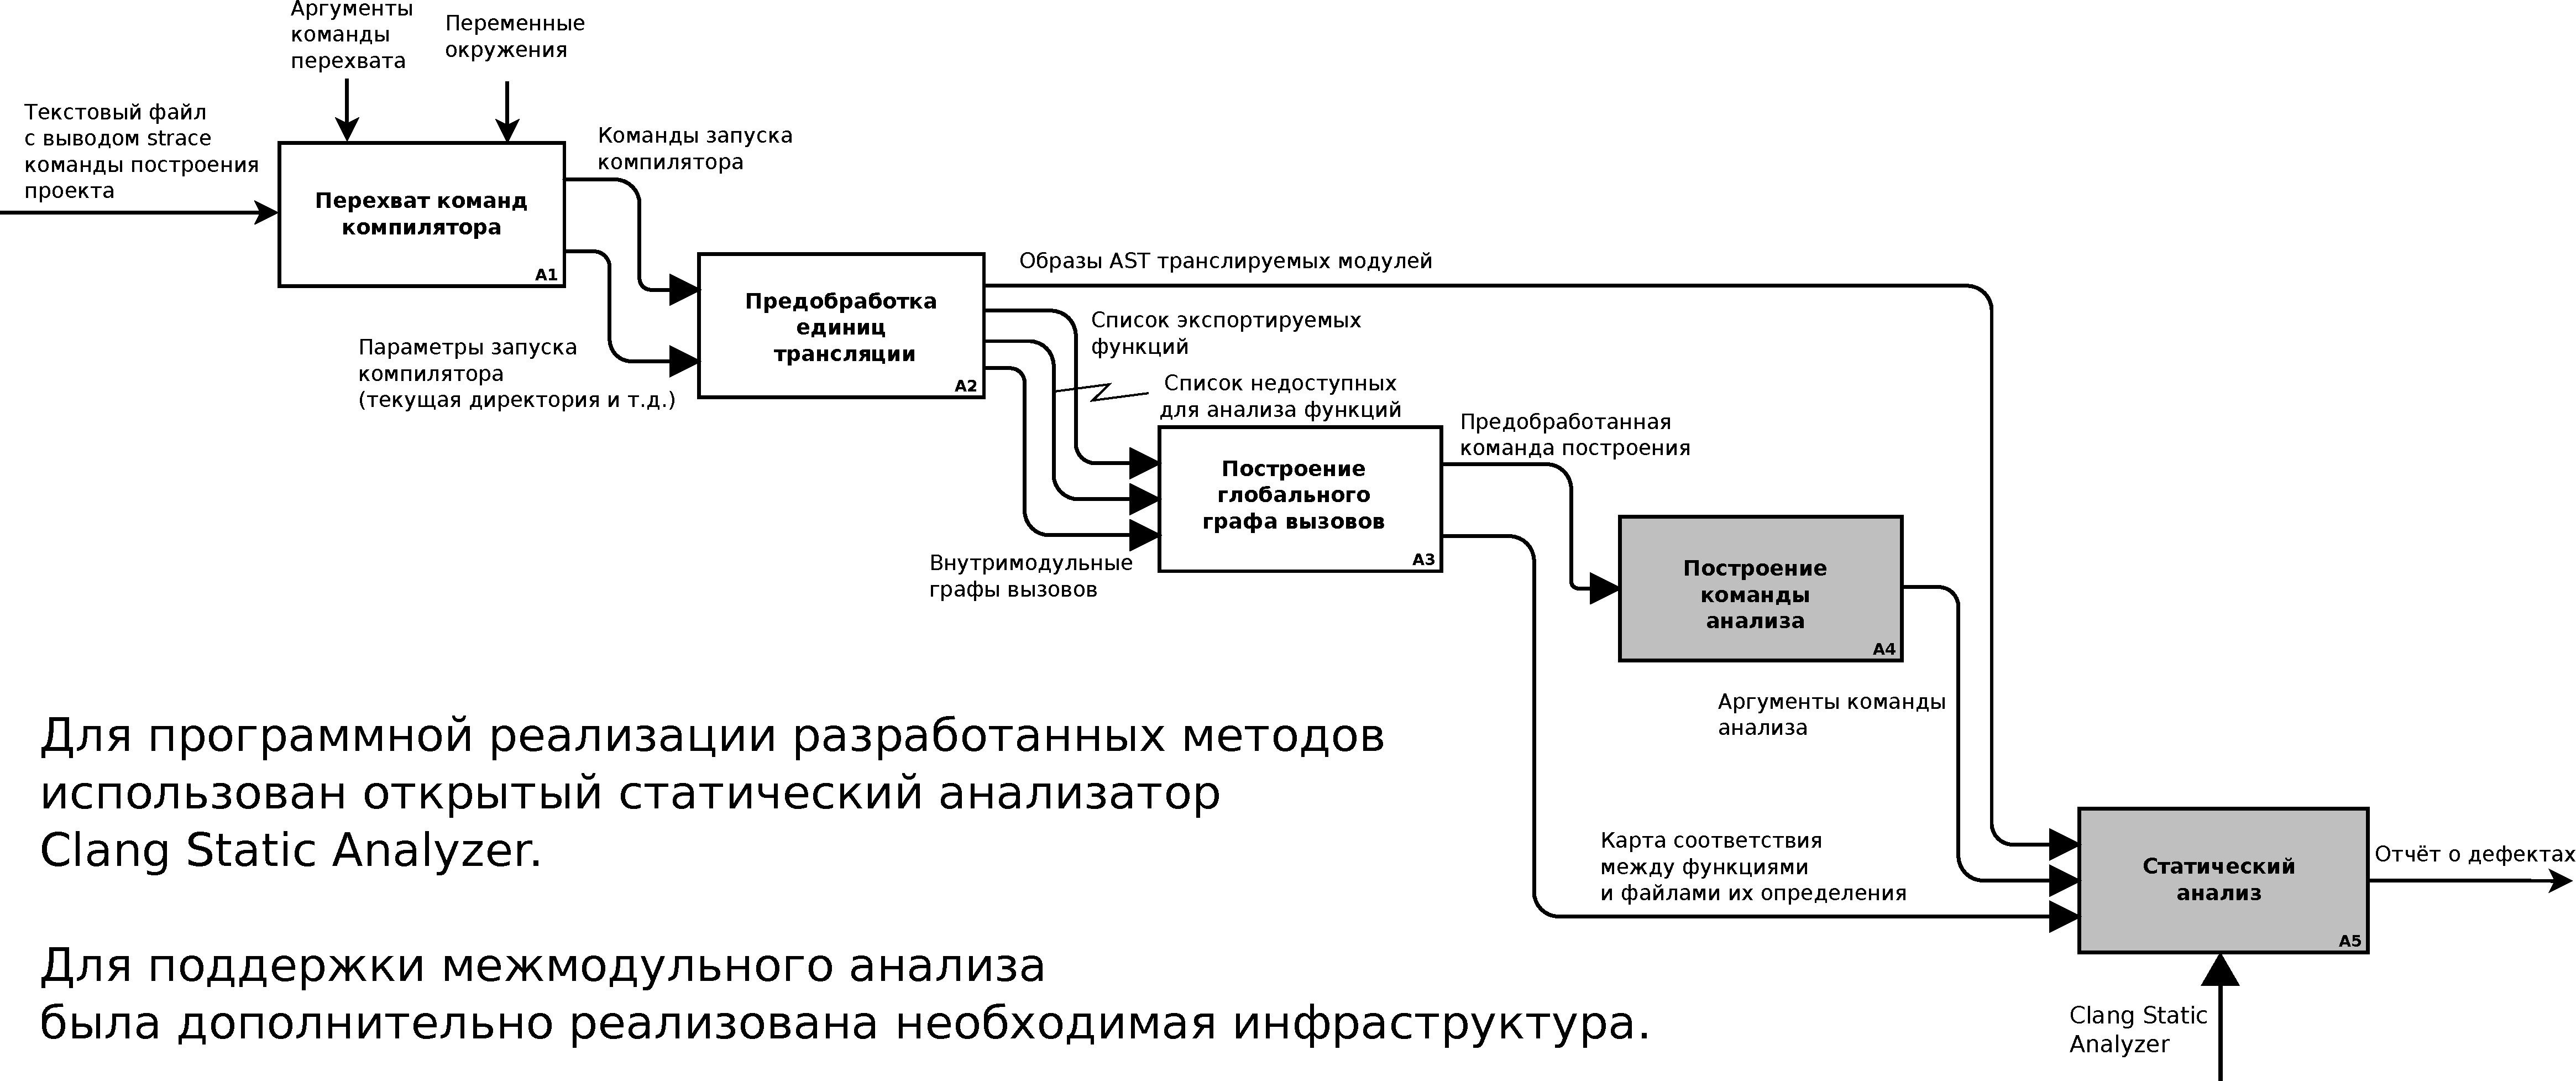
\includegraphics[width=\linewidth]{../Dissertation/images/xtu-idef0-4.pdf}}
\end{figure}
\end{frame}
%--------------------------------------------------------------------------------------------------------

\begin{frame}
\frametitle{Межмодульный анализ}
Разработанные и модифицированные компоненты системы межмодульного анализа.
\begin{figure}[h]
  \center{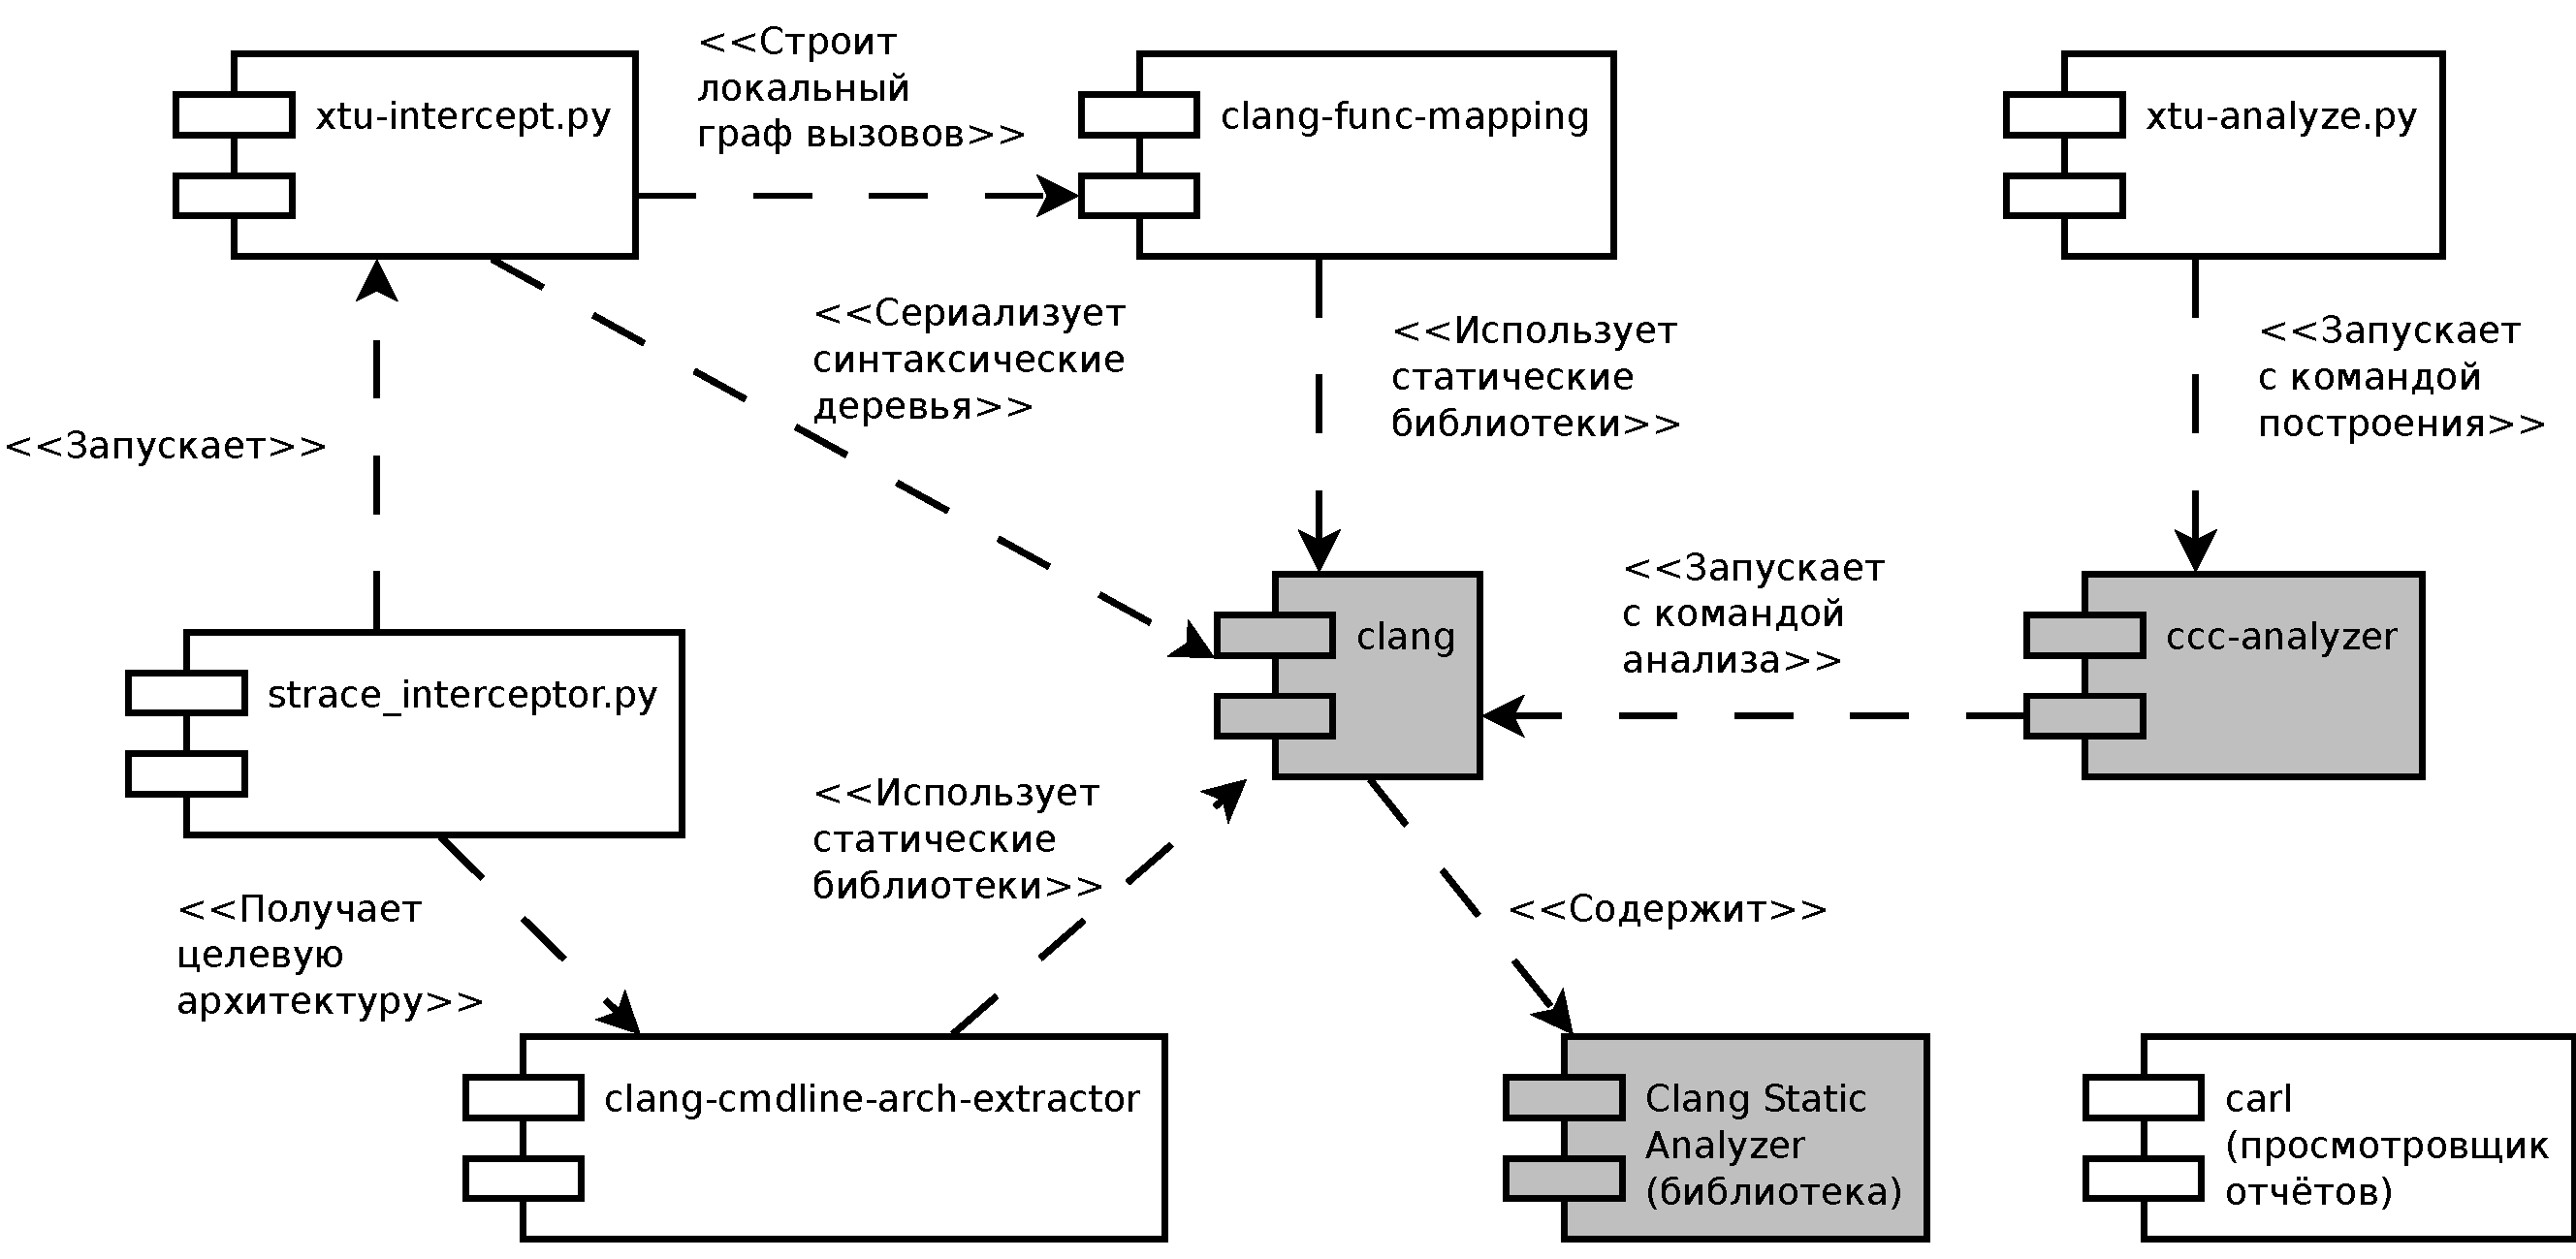
\includegraphics[width=\linewidth]{../Dissertation/images/components.pdf}}
\end{figure}
\end{frame}

%--------------------------------------------------------------------------------------------------------
\begin{frame}
\frametitle{Слияние АСД}
\begin{figure}[h]
  \begin{minipage}[h]{0.49\linewidth}
\begin{itemize}
 \item[+] Прозрачный межмодульный анализ
 \item[+] Возможность выполнения комбинированных проверок
 \item[+] Отсутствие потерь информации о программе
\end{itemize}
  \end{minipage}
  \hfill
  \begin{minipage}[h]{0.49\linewidth}
\begin{itemize}
 \item[--] Проблема конфликтующих определений
 \item[--] Проблема слияния АСД кода, разработанного с использованием различных стандартов языка
\end{itemize}
  \end{minipage}
\end{figure}
\end{frame}

%--------------------------------------------------------------------------------------------------------

\begin{frame}
\frametitle{Анализируемые объёмы кодов программ}
\textbf{Характеристики тестовой базы ОС Android 4.2.1}
\begin{table} [htbp]
  \centering
  \parbox{15cm}{\label{table:android-char}}
%  \begin{center}
  \begin{tabular}{| p{0.7\linewidth} || p{0.2\linewidth} |}
  \hline
  \hline
  \textbf{Характеристика}   & \textbf{Значение} \\
  \hline
  \hline
  Количество строк кода   & 10 млн \\
  \hline
  Количество файлов исходного кода      & 31038    \\
  \hline
  Количество транслируемых модулей  & 20635   \\
  \hline
  Количество архитектур на построение & 2   \\
  \hline
  Количество пакетов & 389 \\
  \hline
  \hline
  \end{tabular}
%  \end{center}
\end{table}
\textbf{Тестовый стенд}
\begin{table} [htbp]
  \begin{tabular}{| p{0.6\linewidth} || p{0.3\linewidth} |}
  \hline
  \hline
  Характеристика   & Значение \\
  \hline
  \hline
  Модель процессора   & Intel Xeon E5-2600 2.60 ГГц \\
  \hline
  Количество физических процессоров & 2   \\
  \hline
  Количество виртуальных ядер системы & 32 (Hyper-Threading)   \\
  \hline
  Оперативная память & 96 Гб DDR3 \\
  \hline
  \hline
  \end{tabular}
%  \end{center}
\end{table}

\end{frame}
%--------------------------------------------------------------------------------------------------------

\begin{frame}
\frametitle{Сравнение методов МПА с использованием разработанного ПО}
Зависимость количества обрабатываемых узлов графа выполнения от времени
\begin{figure}[h]
  \begin{minipage}[h]{0.49\linewidth}
    \center{\textbf{Межмодульный анализ}}
   \center{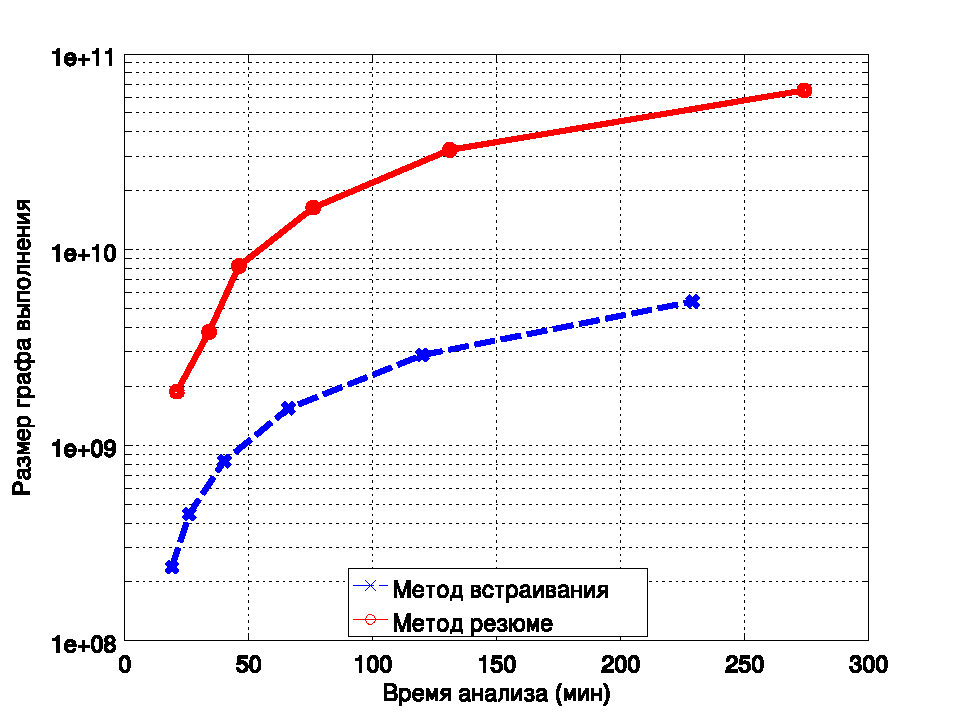
\includegraphics[width=\linewidth]{../Dissertation/images/xtu-nodes.pdf}}
  \end{minipage}
  \hfill
  \begin{minipage}[h]{0.49\linewidth}
    \center{\textbf{Внутримодульный анализ}}
  \center{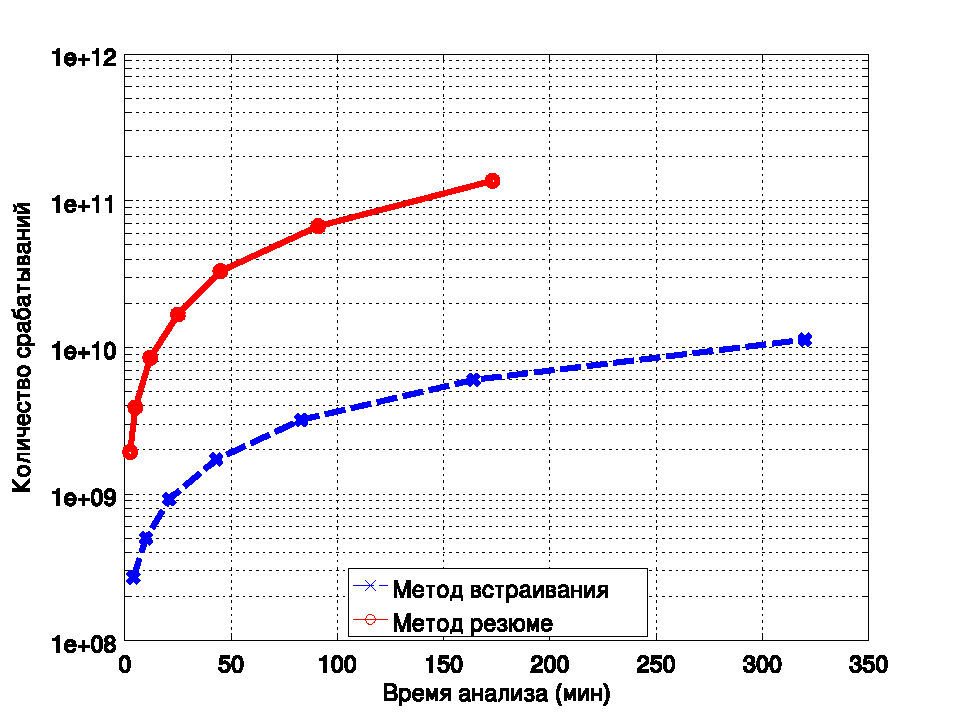
\includegraphics[width=\linewidth]{../Dissertation/images/single-nodes.pdf}}
  \end{minipage}
\end{figure}
\end{frame}

%--------------------------------------------------------------------------------------------------------

\begin{frame}
\frametitle{Сравнение методов МПА с использованием разработанного ПО}
Зависимость количества уникальных отчётов о дефектах от времени
\begin{figure}[h]
  \begin{minipage}[h]{0.49\linewidth}
    \center{\textbf{Межмодульный анализ}}
   \center{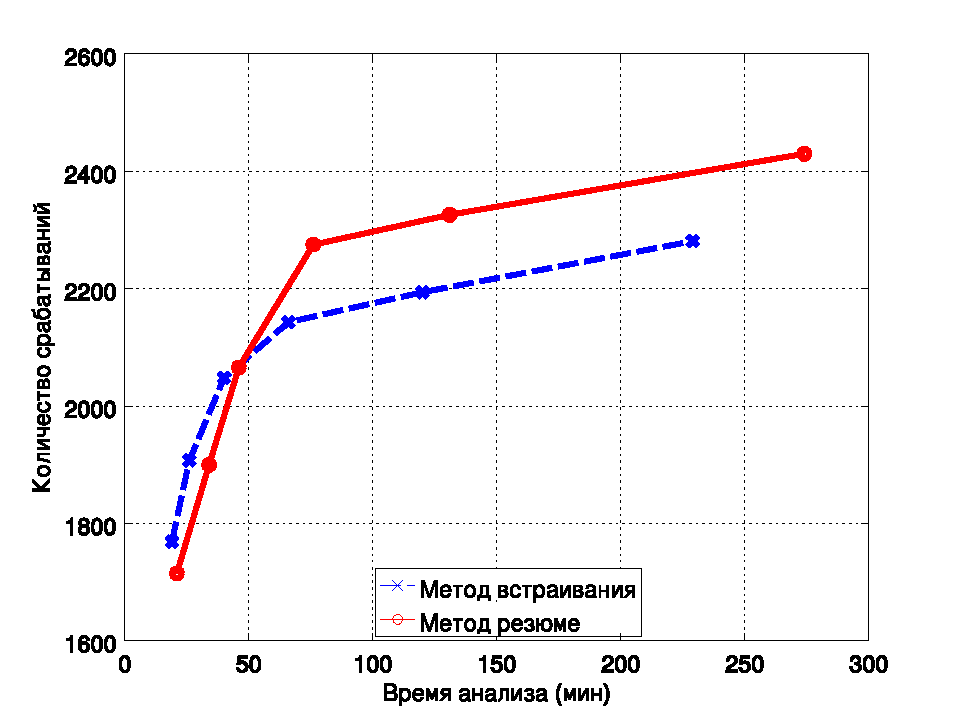
\includegraphics[width=\linewidth]{../Dissertation/images/xtu-unique.pdf}}
  \end{minipage}
  \hfill
  \begin{minipage}[h]{0.49\linewidth}
    \center{\textbf{Внутримодульный анализ}}
  \center{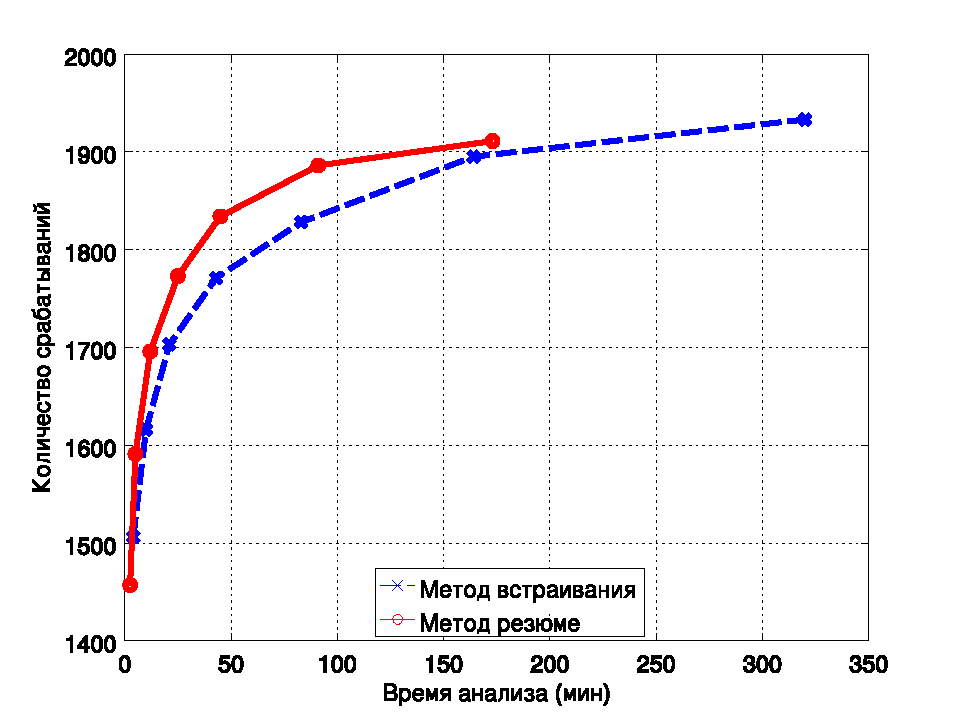
\includegraphics[width=\linewidth]{../Dissertation/images/single-unique.pdf}}
  \end{minipage}
\end{figure}
\end{frame}
%--------------------------------------------------------------------------------------------------------


% \begin{frame}
% \frametitle{Цель работы}
% \begin{itemize}
%   \item Построение метода анализа крупных программных комплексов, разработанных с использованием языков C и C++, способного осуществлять анализ проектов масштаба ОС Android и ОС Tizen (порядка 5--20~млн. строк кода) за приемлемое время и обеспечивающего достаточное покрытие путей выполнения программы.
% \end{itemize}
% \end{frame}
% 
% \begin{frame}
% \frametitle{Актуальные проблемы статического анализа}
% \begin{itemize}
%   \item Необходимость поиска компромисса между качеством, полнотой и временем анализа
%   \item Экспоненциальная сложность наиболее точных и полных видов статического анализа делает их ограниченно применимыми для анализа крупных программных систем
%   \item Проблема улучшения производительности методов статического анализа является актуальной   
% \end{itemize}
% \end{frame}
% 
% \begin{frame}[allowframebreaks]
% \frametitle{Поставленные задачи}
% \begin{enumerate}
%   \item Разработать метод межпроцедурного анализа программ, пригодный для анализа крупных программных проектов, а также расширяемый на различные виды проверок
%   \item Разработать метод межмодульного анализа программ, разработанных с использованием языков C и C++
%   \item Разработать метод отображения результатов анализа при использовании предложенного метода межпроцедурного анализа
%   \item Для экспериментального подтверждения эффективности предложенных методов реализовать их и осуществить тестирование разработанных методов на реальных программных проектах
%   \item По результатам тестирования сделать выводы о пригодности разработанного метода, о его применимости для анализа крупных программных комплексов и качестве анализа кода программ
% \end{enumerate}
% \end{frame}
% 
% \begin{frame}[allowframebreaks]
% \frametitle{Основные положения, выносимые на защиту}
% \begin{enumerate}
%   \item Новая модификация метода межпроцедурного анализа программ на основе резюме для метода символьного выполнения для программ, разработанных с использованием языков C и C++
%   \item Метод межмодульного анализа программ, разработанных с использованием языков C и C++, архитектура анализатора, эвристики, связанные с объединением синтаксических деревьев различных единиц трансляции
%   \item Метод построения отчёта о дефекте при использовании метода резюме для метода символьного выполнения
% \end{enumerate}
% \end{frame}
% 
% \begin{frame}[allowframebreaks]
% \frametitle{Мотивация}
% \begin{itemize}
%   \item Необходимость автоматизации поиска дефектов в крупных и критичных по качеству программных продуктах требует выполнения анализа с высокой полнотой и точностью
%   \item При использовании метода символьного выполнения можно достичь указанных характеристик
%   \begin{itemize}
%     \item Анализ, чувствительный к пути выполнения и потоку управления
%   \end{itemize}
% 
%   \item Для данного метода существует проблема экспоненциального роста количества путей при увеличении размера программы
%   \item Межпроцедурный анализ усугубляет данную проблему, увеличивая количество возможных путей выполнения при использовании контекстно-чувствительного анализа
%   \item Задача разработки метода МПА, в меньшей степени затронутого данной проблемой, является актуальной.
% \end{itemize}
% \end{frame}
% 
% \begin{frame}[allowframebreaks]
% \frametitle{Мотивация~--- языки программирования C и C++}
% \begin{itemize}
%   \item Большое количеством видов потенциальных ошибок, которые может допустить программист
%   \begin{itemize}
%     \item Неправильная работа с~указателями
%     \item Неопределённое или зависящее от реализации поведение
%   \end{itemize}
%   \item Наиболее распространённые и~известные языки
%     \begin{itemize}
%     \item Большое количество существующего системного и~прикладного ПО
%     \item ПО с высокими требованиями к производительности
%     \item Низкоуровневые компоненты, такие как компоненты операционных систем и~драйверы
%   \end{itemize}
%   \item Проблема глубокого анализа программ на языках C и C++ является актуальной.
% \end{itemize}
% \end{frame}
% 
% \begin{frame}[allowframebreaks]
% \frametitle{Предлагаемая модификация метода резюме}
% \begin{itemize}
%   \item Анализ функции вне контекста вызова с последующим уточнением контекста
%   \item Позволяет не анализировать одну и ту же функцию многократно, а использовать её резюме
%   \item Использовался различными исследователями для реализации обособленных видов проверок
% \end{itemize}
% \end{frame}
% 
% \begin{frame}[allowframebreaks]
% \frametitle{Предлагаемая модификация метода резюме}
% \begin{itemize}
%   \item Цель исследования: построение многоцелевого анализатора для языков C и C++
%   \item Решённые проблемы:
%   \begin{itemize}
%     \item Поддержка модели памяти C/C++, включая арифметику указателей, наследования и выравнивания полей структур
%     \item Отсечение недостижимых путей выполнения
%     \item Поддержка сложных алгоритмов поиска дефектов и их одновременного использования при МПА методом резюме
%   \end{itemize}
% \end{itemize}
% \end{frame}
% 
% \begin{frame}
% \frametitle{Структура резюме}
% \begin{itemize}
%   \item В предлагаемой модификации, \textit{резюме} представляет собой набор \textit{ветвей резюме}, каждая из которых соответствует листу графа выполнения функции
%   \item Соответственно, каждая ветвь задаёт класс эквивалентности относительно параметров функции
%   \item Каждая ветвь содержит предусловия, при которых достижима данная ветвь, и постусловие, которое является эффектом ветви выполнения функции на состояние программы.
% \end{itemize}
% \end{frame}
% 
% \begin{frame}
% \frametitle{Поддержка модели памяти в резюме}
% \begin{itemize}
%   \item Для анализа функции в контексте вызова производится \textit{актуализация} символьных значений
%   \begin{enumerate}
%     \item Вне контекста строится цепочка доступа вида \\ \textit{<<параметр функции 1 $\rightarrow$ поле lock $\rightarrow$ элемент 2>>}
%     \item В контексте вызова цепочка доступа применяется к региону памяти, являющемуся фактическим аргументом при вызове функции
%   \end{enumerate}
% \end{itemize}
% \end{frame}
% 
% \begin{frame}[allowframebreaks]
% \frametitle{Применение резюме. Отсечение недостижимых путей}
% \begin{itemize}
%   \item Каждое символьное значение имеет своё множество возможных конкретных значений
%   \item Пересечение этих диапазонов для фактических и формальных параметров становится новым диапазоном конкретных значений фактического параметра в вызывающей функции
%   \item Пустое пересечение означает недостижимость данной ветви выполнения
%   \item Если ветвь выполнения достижима, применяются постусловия, включающие в себя привязку новых символьных значений к регионам памяти, в которые произошла запись в вызываемой функции
%   \item Символьное значение, возвращаемое функцией, также подвергается актуализации и становится значением выражения-вызова функции.
% \end{itemize}
% \end{frame}
% 
% \begin{frame}[allowframebreaks]
% \frametitle{Проверки при применении резюме}
% \begin{itemize}
%   \item Каждый проверяющий модуль имеет своё состояние (type state)
%   \item Каждый проверяющий модуль может создавать своё резюме и применять его независимо как от других модулей, так и от остальных компонентов анализатора, что позволяет реализовывать МПА методом резюме для проверок произвольного вида
%   \item В резюме проверяющего модуля обычно входят изменения состояния программы и отложенные проверки
%   \item В рамках данной работы МПА методом резюме был реализован для проверяющих модулей различного назначения:
%     \begin{itemize}
%     \item Строковое переполнение
%     \item Корректность операций над файловыми дескрипторами
%     \item Проверка корректности синхронизации в многопоточной среде
%     \item Целочисленное переполнение
%     \item Запись в переменную константного типа
%   \end{itemize}
% \end{itemize}
% \end{frame}
% 
% \begin{frame}
% \frametitle{Построение отчёта}
% \begin{itemize}
%   \item Отчёт должен содержать полную информацию о пути выполнения, на котором наблюдается дефект
%   \item При использовании метода резюме происходит потеря информации о пути выполнения внутри вызываемой функции
%   \item Для решения этой проблемы предлагается использовать хранение ссылки на узел графа вызываемой функции, соответствующий ветви применения резюме.
% \end{itemize}
% \end{frame}

% \begin{frame}
% \frametitle{Межмодульный анализ}
% \begin{itemize}
%   \item C и C++~--- языки с поддержкой раздельной компиляции
%   \item Для анализа крупных программ необходимо обрабатывать функции, определённые в различных единицах трансляции
%   \item Для решения этой проблемы предлагается использовать слияние синтаксических деревьев единиц трансляции.
%     \begin{itemize}
%       \item Данный метод позволяет сохранять всю доступную информацию о программе без потери при преобразованиях
%     \end{itemize}
% \end{itemize}
% \end{frame}
% 
% \begin{frame}
% \frametitle{Межмодульный анализ~--- реализация}
% В данной работе реализован межмодульный анализ, состоящий из трёх фаз
% \begin{enumerate}
%   \item На первой фазе происходит перехват команд построения проекта
%   \begin{enumerate}
%     \item Построение синтаксических деревьев единиц трансляции с сохранением их на носитель
%     \item Сохранение данных о требуемых и имеющихся определениях функций
%   \end{enumerate}
%   \item На второй фазе строится соответствие между требуемыми и имеющимися функциями, производится топологическая сортировка графа вызовов
%   \item На третьей фазе происходит запуск анализа со слиянием синтаксических деревьев.
% \end{enumerate}
% \end{frame}
% 
% \begin{frame}[allowframebreaks]
% \frametitle{Межмодульный анализ~--- решаемые проблемы}
% \begin{enumerate}
%   \item Необходимость различения синтаксических деревьев и функций различных архитектур, а также перегруженных функций
%     \begin{itemize}
%       \item Для поиска используются сигнатуры, содержащие соответствующую информацию
%     \end{itemize}
%   \item Длительный рекурсивный поиск
%   \begin{enumerate}
%     \item Объявления с различными именами являются различными
%     \item Объявления различных разновидностей являются различными
%     \item Объявления из одного файла с одинаковыми текстовыми позициями начала и завершения считаются совпадающими
%   \end{enumerate}
%   \item Сложные зависимости между импортируемыми объявлениями при рекурсивном импорте
%     \begin{itemize}
%       \item Необходимо переупорядочивать сливаемые объявления
%     \end{itemize}
% \end{enumerate}
% \end{frame}

% 
% \begin{frame}
% \frametitle{Покрытие~--- внутримодульный анализ}
% \begin{figure}[h]
%   \center{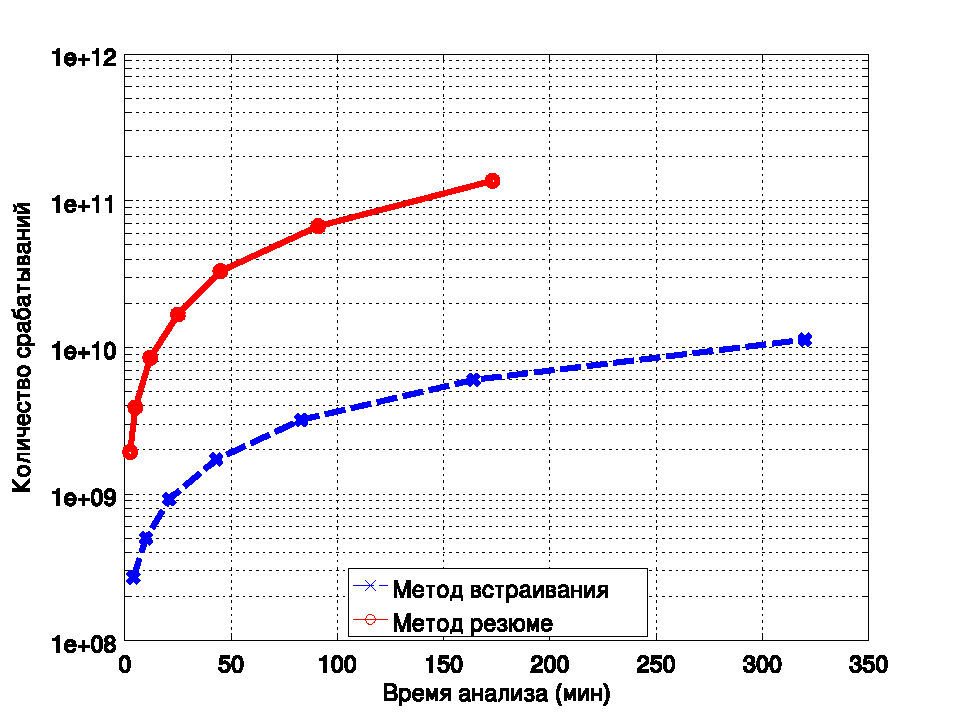
\includegraphics[width=0.8\linewidth]{../Dissertation/images/single-nodes.pdf}}
% \end{figure}
% \end{frame}
% 
% \begin{frame}
% \frametitle{Покрытие~--- межмодульный анализ}
% \begin{figure}[h]
%   \center{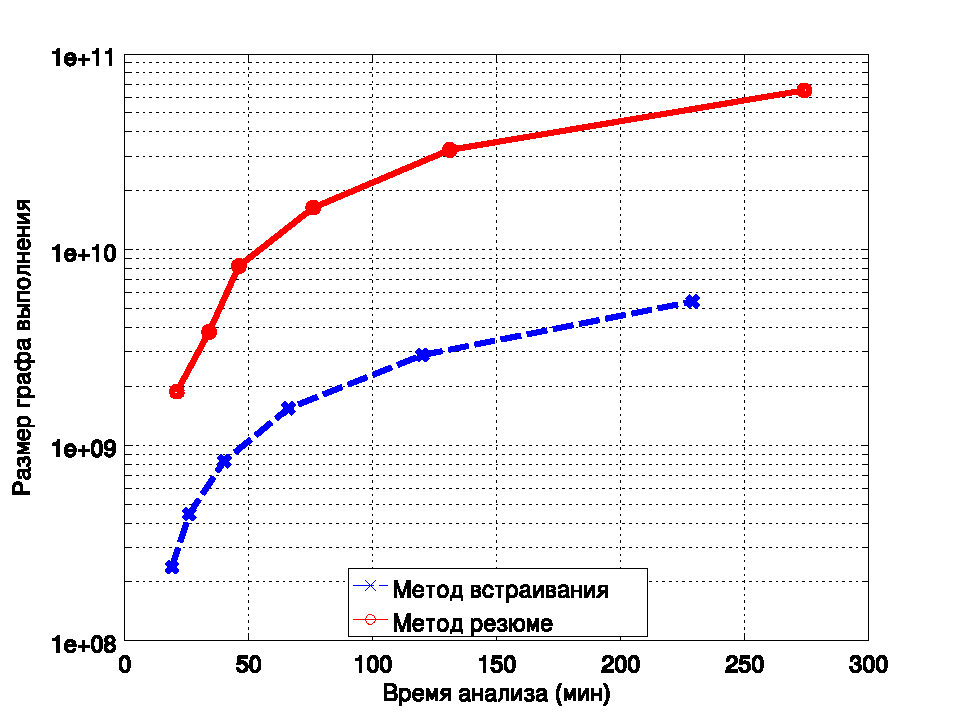
\includegraphics[width=0.8\linewidth]{../Dissertation/images/xtu-nodes.pdf}}
% \end{figure}
% \end{frame}
% 
% \begin{frame}
% \frametitle{Поиск дефектов~--- внутримодульный анализ}
% \begin{figure}[h]
%   \center{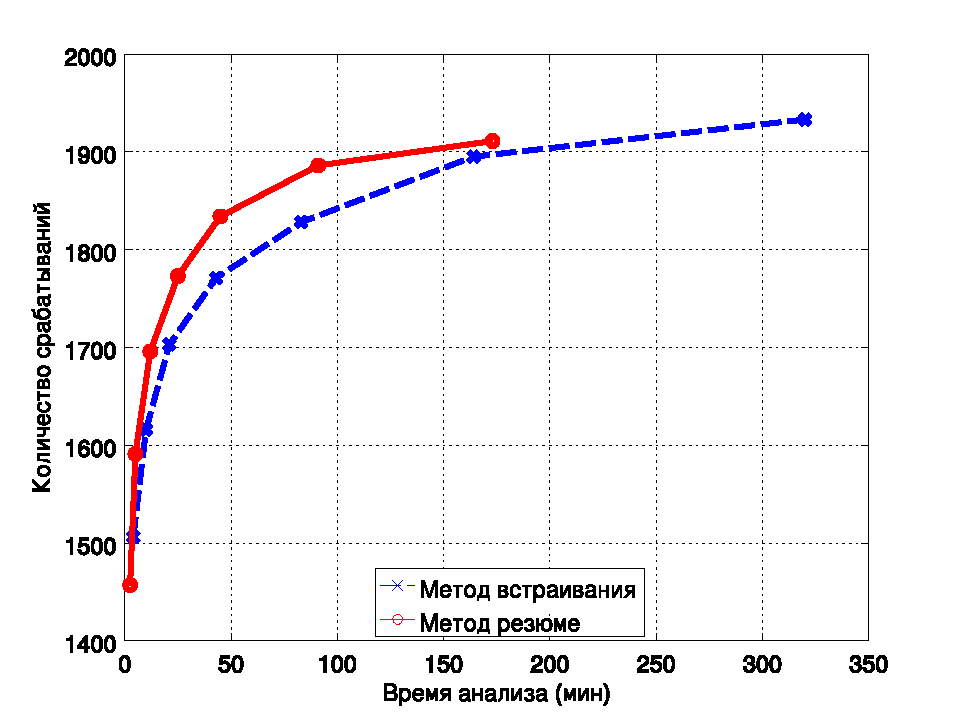
\includegraphics[width=0.8\linewidth]{../Dissertation/images/single-unique.pdf}}
% \end{figure}
% \end{frame}
% 
% \begin{frame}
% \frametitle{Поиск дефектов~--- межмодульный анализ}
% \begin{figure}[h]
%   \center{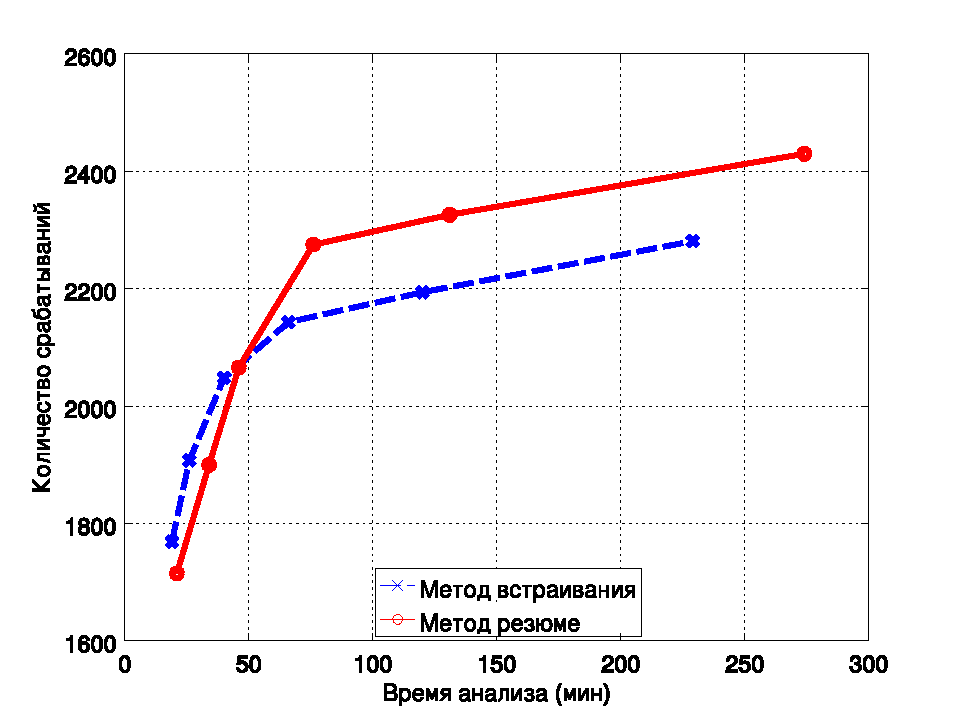
\includegraphics[width=0.8\linewidth]{../Dissertation/images/xtu-unique.pdf}}
% \end{figure}
% \end{frame}
%--------------------------------------------------------------------------------------------------------

\begin{frame}
\frametitle{C/C++ пакеты системы Android 4.2.1~---\\диаграмма связей}
\begin{figure}[h]
  \center{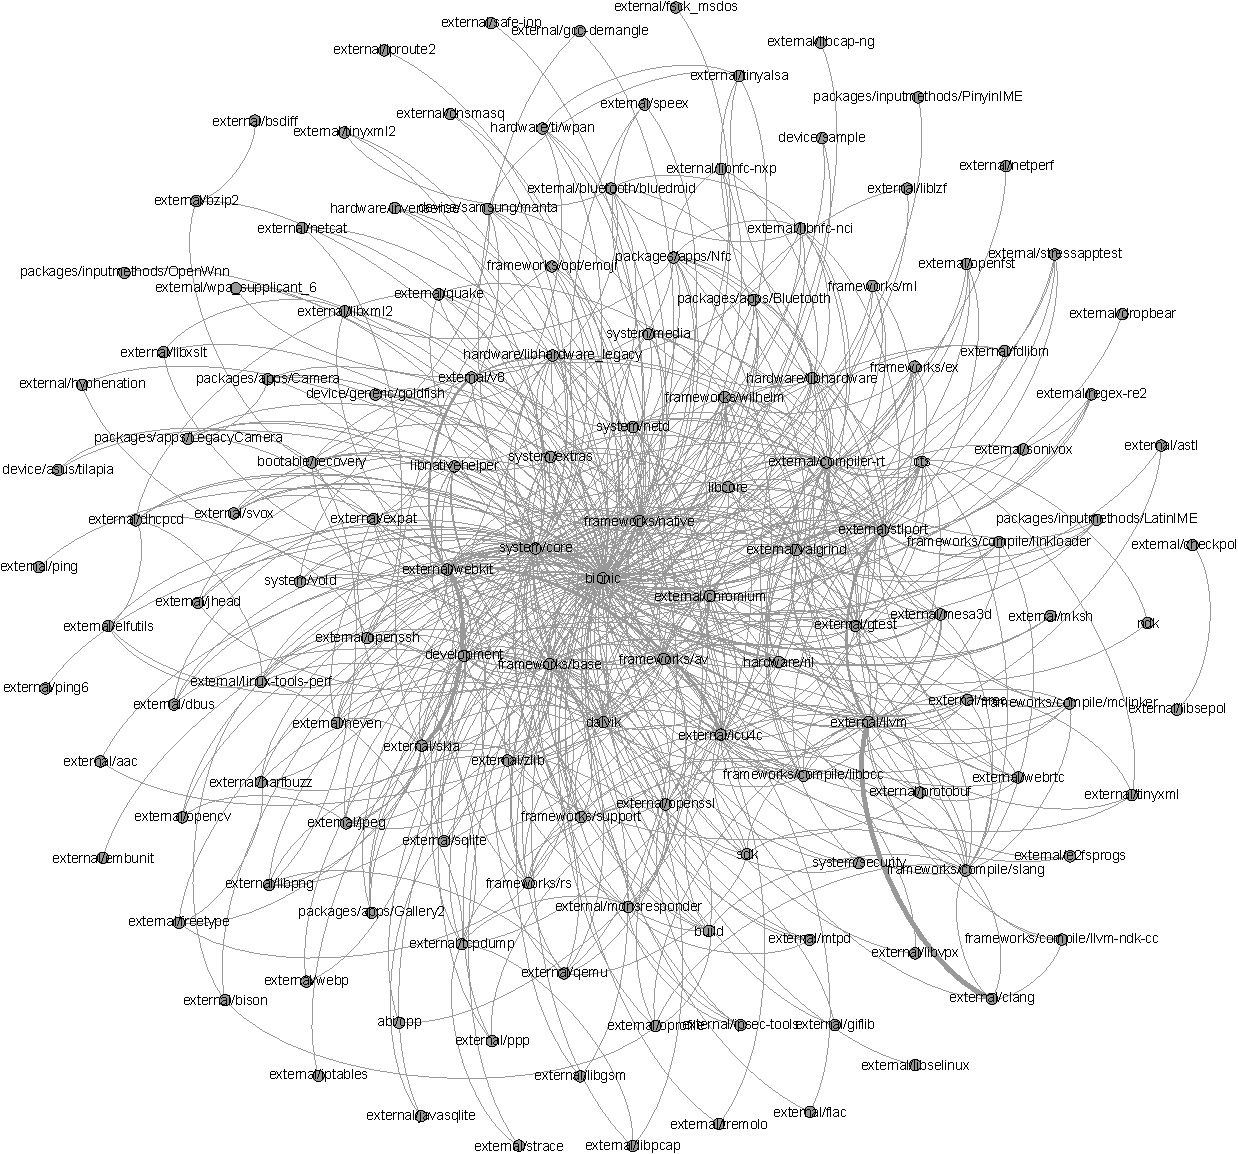
\includegraphics[height=0.65\linewidth]{../Dissertation/images/callgraph.pdf}}
\end{figure}
\end{frame}

%--------------------------------------------------------------------------------------------------------

\begin{frame}[allowframebreaks]
\frametitle{Научные результаты, представляемые на защиту}
\begin{enumerate}
  \item Продемонстрирован значительный рост производительности анализа
  \item Покрытие операторов программы увеличилось в 10--15 раз
  \item Скорость поиска дефектов также увеличилась: то же количество уникальных дефектов можно обнаружить в 2--3 раза быстрее
  \item Точность анализа сохранилась и составила от 80\% до 84\%
\end{enumerate}
\end{frame}
%%%%%%%%%%%%%%%%%%%%%%%%%%%%%%
\begin{frame}
\frametitle{Перспективы развития методов и ПО, разработанного на их основе}
\begin{itemize}
  \item Исследование и реализация возможностей повторного использования резюме при межмодульном анализе с целью увеличения быстродействия процесса анализа
  \item Использование методов, применяемых компоновщиками, для поиска требуемых определений функций с целью улучшения корректности межмодульного анализа в рамках разработанного ПО
  \item Реализация МПА методом резюме для большего количества проверяющих модулей, включая проверки безопасности, с целью дальнейшего внедрения и промышленного применения результирующего ПО. 
\end{itemize}
\end{frame}
% 
% \begin{frame}[allowframebreaks]
% \frametitle{Результаты работы}
% \begin{itemize}
%   \item Разработана новая модификация метода межпроцедурного анализа программ на основе резюме для метода символьного выполнения для программ, реализованных с использованием языков C и C++. Данный метод анализа позволяет производить анализ с высоким качеством и полнотой, однако имеет экспоненциальную сложность, связанную с проблемой роста количества путей с увеличением объёма программы (path explosion), что делает задачу улучшения его производительности особенно актуальной. Важными особенностями разработанного метода является поддержка проверок произвольного вида и их одновременного выполнения, а также поддержка модели памяти, используемой в языках C и C++, в том числе, с учётом арифметики указателей, наследования и выравнивания полей структур.
%   \item Разработан метод межмодульного анализа программ, реализованных с использованием языков C и C++ для статического анализатора, использующего в качестве входных данных непосредственно исходный код программы. Использование промежуточного представления в виде синтаксического дерева программы позволяет производить анализ без потери информации о программе.
%   \item Разработан метод построения отчёта о дефекте при использовании предложенной модификации метода резюме для метода символьного выполнения. Данный метод позволяет строить информативный межпроцедурный отчёт, включающий показ переходов, выполнимых условий и представляющих интерес событий в процессе выполнения программы.
%   \item Для экспериментального подтверждения эффективности предложенных методов они были реализованы их для использования в приложении-анализаторе (Clang Static Analyzer, анализатор с открытым исходным кодом). Было осуществлено тестирование разработанных методов на реальных программных проектах~--- пакетах пользовательского окружения ОС Android.
%   \item По результатам тестирования сделан выводы о пригодности разработанного метода. Несмотря на сохранение экспоненциальной сложности анализа, тесты показали, что скорость поиска дефектов и покрытие путей тестируемых программы увеличились, а качество анализа кода программ сохранилось на том же уровне.
% \end{itemize}
% \end{frame}
% 
% %--------------------------------------------------------------------------------------------------------
% %TODO: Убрать за ``Спасибо'', сделать запасным.
% \begin{frame}[allowframebreaks]
% \frametitle{Решаемые задачи}
% 
% \begin{enumerate}
%   \item Исследование областей применения и функциональных особенностей систем статического анализа кодов программ для формализации подхода к модификации метода с целью уменьшения времени анализа.
%   \item Разработка модификации метода межпроцедурного анализа программ, пригодной для реализации в многоцелевом статическом анализаторе программного кода на языках C и C++ и позволяющей использовать различные виды проверок кода с целью поиска дефектов.
%   \item Теоретическое обоснование возможности применения разрабатываемой модификации метода для применения в автоматизированной системе тестирования.
%   \item Разработка математической модели для оценки корректности применения разработанного подхода к анализу программ.
%   \item Разработка метода межмодульного анализа программ, разработанных с использованием языков C и C++, для повышения полноты анализа многокомпонентных систем.
%   \item Разработка метода отображения результатов анализа при использовании предложенного метода межпроцедурного анализа с целью уменьшения времени на воспроизведение и исправление обнаруженных дефектов.
%   \item Реализация предложенных методов для использования в приложении-анализаторе (Clang Static Analyzer, анализатор с открытым исходным кодом) с целью экспериментального подтверждения их эффективности и тестирование разработанных методов на реальных программных проектах~--- пакетах пользовательского окружения ОС Android.
% \end{enumerate}
% 
% \end{frame}
%--------------------------------------------------------------------------------------------------------

% \begin{frame}
% \frametitle{Формулы}
% $$
% \left\{
%   \begin{array}{rl}
%     \dot x = & \sigma (y-x) \\
%     \dot y = & x (r - z) - y \\
%     \dot z = & xy - bz
%   \end{array}
% \right.
% $$
% \end{frame}
% 
% \begin{frame}
% \frametitle{Составное изображение}
% \begin{figure}[h]
%   \begin{minipage}[h]{0.49\linewidth}
%     \textbf{Составная \\ подпись 1}
%     \center{\includegraphics[width=1\linewidth]{knuth1}}
%   \end{minipage}
%   \hfill
%   \begin{minipage}[h]{0.49\linewidth}
%     \textbf{Составная \\ подпись 2}
%     \center{\includegraphics[width=1\linewidth]{knuth2}}
%   \end{minipage}
% \end{figure}
% \end{frame}
% 
% \begin{frame}
% \frametitle{Таблица}
% \begin{tabular}{|l|l|}
% \hline
% \textbf{Заголовок 1} & \textbf{Заголовок 2} \\
% \hline
% Сумма & $b+a$ \\
% \hline
% Разность & $a-b$ \\
% \hline
% Произведение & $a*b$ \\
% \hline
% \end{tabular}
% \end{frame}
% 
% \begin{frame}
% \frametitle{Большой многоуровневый список}
% \begin{itemize}
%   \item \textbf{Пункт 1}
%     \begin{itemize}
%       \itemi Подпункт 1-1
%       \itemi Подпункт 1-2
%     \end{itemize}
%   \item \textbf{Пункт 2}
%     \begin{itemize}
%       \itemi Подпункт 2-1
%     \end{itemize}
%   \item \textbf{Пункт 3}
%     \begin{itemize}
%       \itemi Подпункт 3-1
%       \itemi Подпункт 3-2
%     \end{itemize}
%   \item \textbf{Пункт 4}
%     \begin{itemize}
%       \itemi Подпункт 4-1
%     \end{itemize}
%   \item \textbf{Пункт 5}
%     \begin{itemize}
%       \itemi Подпункт 5-1
%       \itemi Подпункт 5-2
%       \itemi Подпункт 5-3
%     \end{itemize}
% \end{itemize}
% \end{frame}
% 
% \begin{frame}
% \frametitle{Четыре изображения}
% \begin{figure}[H]
%   \center
%     \includegraphics[width=0.4\linewidth]{latex}
%     \includegraphics[width=0.4\linewidth]{latex}\\
%     \includegraphics[width=0.4\linewidth]{latex}
%     \includegraphics[width=0.4\linewidth]{latex}
% \end{figure}
% \end{frame}


\end{document} 